\documentclass[11pt,a4paper,oldfontcommands]{memoir}
\usepackage[utf8]{inputenc}
\usepackage[T1]{fontenc}
\usepackage{microtype}
\usepackage[dvips]{graphicx}
\usepackage{xcolor}
\usepackage{todonotes}
\usepackage{times}
\usepackage{amsmath}
\usepackage{natbib}
\usepackage{array}
\usepackage{listings}
\usepackage{pgf-umlsd}
\usepackage{parskip}

\setlength{\parskip}{10pt} %add space between paragraphs

%%% Fix the issue with \mess redefinition when importing msc
\let\msg\mess
\let\mess\undefined

\newcommand\draft{1}

\if1\draft
    \overfullrule=2cm
\fi

\lstset{
  language = C,
  basicstyle=\small,    % the size of the fonts that are used for the code
  stepnumber=1,                           % the step between two line-numbers. If it is 1 each line will be numbered
  numbersep=10pt,                         % how far the line-numbers are from the code
  tabsize=2,                              % tab size in blank spaces
  extendedchars=true,                     %
  breaklines=true,                        % sets automatic line breaking
  captionpos=b,                           % sets the caption-position to top
  mathescape=true,
  stringstyle=\color{white}\ttfamily,
  showspaces=false,           
  showtabs=false,             
  xleftmargin=17pt,
  framexleftmargin=17pt,
  framexrightmargin=17pt,
  framexbottommargin=5pt,
  framextopmargin=5pt,
  showstringspaces=false     
 }

\renewcommand\lstlistlistingname{List of Listings}
\newlistof{lstlistoflistings}{lol}{\lstlistlistingname}
\newcommand\typestyle{\rmfamily\mdseries\upshape}
\newcommand\addtypes[1]{%
  \lstset{morekeywords=[3]{#1}}}

\usepackage[
breaklinks=true,colorlinks=true,
%linkcolor=blue,urlcolor=blue,citecolor=blue,% PDF VIEW
linkcolor=black,urlcolor=black,citecolor=black,% PRINT
bookmarks=true,bookmarksopenlevel=2]{hyperref}

\usepackage{breakurl}

\usepackage{geometry}
% PDF VIEW
% \geometry{total={210mm,297mm},
% left=25mm,right=25mm,%
% bindingoffset=0mm, top=25mm,bottom=25mm}
% PRINT
\geometry{total={210mm,297mm},
left=20mm,right=20mm,
bindingoffset=10mm, top=25mm,bottom=25mm}

\usepackage{bytefield}
\usepackage{msc}

\OnehalfSpacing
%\linespread{1.3}

%%% CHAPTER'S STYLE
\chapterstyle{bianchi}
%\chapterstyle{ger}
%\chapterstyle{madsen}
%\chapterstyle{ell}
%%% STYLE OF SECTIONS, SUBSECTIONS, AND SUBSUBSECTIONS
\setsecheadstyle{\Large\bfseries\sffamily\raggedright}
\setsubsecheadstyle{\large\bfseries\sffamily\raggedright}
\setsubsubsecheadstyle{\bfseries\sffamily\raggedright}


%%% STYLE OF PAGES NUMBERING
%\pagestyle{companion}\nouppercaseheads 
%\pagestyle{headings}
%\pagestyle{Ruled}
\pagestyle{plain}\nouppercaseheads
\makepagestyle{plain}
\if0\draft
\makeevenfoot{plain}{\thepage}{Multipath DTLS: Design and Implementation}{}
\makeoddfoot{plain}{}{Q. Devos \& L. Fortemps de Loneux}{\thepage}
\makeevenhead{plain}{\leftmark}{}{}
\makeoddhead{plain}{}{}{\rightmark}
\else
\makeevenfoot{plain}{\thepage}{}{}
\makeoddfoot{plain}{}{}{\thepage}
\makeevenhead{plain}{}{}{}
\makeoddhead{plain}{}{}{}
\fi

\maxsecnumdepth{subsection} % chapters, sections, and subsections are numbered
\maxtocdepth{subsection} % chapters, sections, and subsections are in the Table of Contents


%%%---%%%---%%%---%%%---%%%---%%%---%%%---%%%---%%%---%%%---%%%---%%%---%%%

\begin{document}
%%%---%%%---%%%---%%%---%%%---%%%---%%%---%%%---%%%---%%%---%%%---%%%---%%%
%   TITLEPAGE
%
%   due to variety of titlepage schemes it is probably better to make titlepage manually
%
%%%---%%%---%%%---%%%---%%%---%%%---%%%---%%%---%%%---%%%---%%%---%%%---%%%
\if0\draft
\thispagestyle{empty}

{%%%
\sffamily
\centering
\Large

~\vspace{\fill}

EPL-2014 384\\
{\huge 
Multipath DTLS: Design and Implementation
}

\vspace{2.5cm}

{\LARGE
Quentin Devos \\
Loïc Fortemps de Loneux
}

\vspace{3.5cm}

A thesis submitted in partial fulfillment for the\\
Master in Computer Science Engineering\\[1em]
in the\\[1em]
Louvain School of Engineering\\
Université Catholique de Louvain

\vspace{3.5cm}

Supervisors: \\
Prof. Olivier Bonaventure\\
Prof. Olivier Pereira

\vspace{\fill}

June 2015

%%%
}%%%

\cleardoublepage
%%%---%%%---%%%---%%%---%%%---%%%---%%%---%%%---%%%---%%%---%%%---%%%---%%%
%%%---%%%---%%%---%%%---%%%---%%%---%%%---%%%---%%%---%%%---%%%---%%%---%%%

\tableofcontents*
\clearpage

\listoffigures*
\clearpage

\lstlistoflistings*
\clearpage

%%%---%%%---%%%---%%%---%%%---%%%---%%%---%%%---%%%---%%%---%%%---%%%---%%%
%%%---%%%---%%%---%%%---%%%---%%%---%%%---%%%---%%%---%%%---%%%---%%%---%%%

%\chapter{Introduction}

Hello, this is fuck**g good thesis, please read !
%\include{rpc}
%\chapter{Protocol Design}

In this chapter, we will explore the different additions and modifications made to DTLS to support the Multi Path capability. These changes are categorized in three groups:
\begin{itemize}
\item Advertising the extension and the interfaces
\item Establishing secure sub-flows without introducing attacks vectors
\item Gathering and exchanging statistics data about the health of each flows, regardless of the others. 
\end{itemize}


\section{Multi-Path advertisement}

Our main purpose is to establish this protocol as an extension of DTLS. In this way, we can reuse as much as possible the principles established by Rescorla and Modadugu in \cite{modadugu2004design}. This also explains why we tried not to change the existing DTLS frames and instead to add new frames for new usages.

\subsection{Extension discovery}

The first step, and the first requirement, was to remain compatible with the standard DTLS client and server. To do that, the MPDTLS extension discovery is made through a new entry in the extensions list of the \verb!ClientHello! and \verb!ServerHello! messages. If a non-MPDTLS capable server receives a \verb!ClientHello!, it will ignore the option  as it is specified in the TLS 1.2 specifications (\verb!RFC5246!\cite{rfc5246}). This option is carried as any other TLS Hello Extension (Section 7.4.1.4 from the same RFC).

This extension is simply carrying a byte indicating if the host supports MPDTLS or not (so it carry \verb!0x01! or \verb!0x00! respectively).\\

After the exchange of the \verb!HelloVerifyRequest! and \verb!ClientHello! with Cookie, the server will send back a \verb!ServerHello! containing the same extension if it wants to support MPDTLS features. Besides this MPDTLS extension discovery, the handshake is exactly the one from DTLS, keeping the handshake as light as possible.

\subsection{Interfaces advertising}

Once the handshake is finished and the initial flow is established, the two hosts can advertise new interfaces available for other sub-flows. This advertising is done within the \verb!ChangeInterfaceMessage! (CIM), a packet carrying multiple addresses. The address of each available interface is included under the form presented in Figure \ref{fig:cimFormat}. We use 16 bytes for the address to be IPv6 compliant. IPv4 addresses can be mapped to/from IPv6 format following \verb!RFC4291!\cite{rfc4291}.  

\begin{figure}[!h]
\centering
\begin{bytefield}[bitwidth=\linewidth/20]{18}
\bitbox{16}{Address} & \bitbox{2}{Port}\\
\bitbox[]{16}{16 bytes} & \bitbox[]{2}{2 bytes}
\end{bytefield}
\caption{Change Interface Message : address format}
\label{fig:cimFormat}
\end{figure}

The \verb!CIM! contains all the addresses a host want to share. We decided to always transmit all the addresses to provide redundancy. Also, to be sure that we does not loose potential bandwidth, the \verb!CIM!s are retransmitted in case of loss and so are acknowledged. To avoid wasting resources, we use the acknowledgement to transmit the list of addresses of the receiving host. This way, we are sure that each host knows the exact configuration of the other at any time (once the first host received the acknowledgement). An example of the \verb!CIM! exchange is shown in the Figure \ref{fig:CIMexchange}.

\begin{figure}[!h]
\centering
\begin{msc}[r]{MultiPath-DTLS Addresses announcement}

\setlength{\instfootheight}{0em}
\setlength{\instheadheight}{0em}
\setlength{\instdist}{0.7\linewidth}
\setlength{\levelheight}{3em}

\declinst{client}{Client}{}
\declinst{server}{Server}{}

\lost[r]{ChangeInterfaceMessage[2, client1, client2, reply=1]}[t]{}{client}[7]
\settimeout{}{client}[1]
\nextlevel
\mess{ChangeInterfaceMessage[2, client1, client2, reply=1]}[t]{client}[0]{server}[1]
\nextlevel
\mess{ChangeInterfaceMessage[1, server1, [reply=0]]}[b]{server}[1]{client}[1]
\nextlevel
\nextlevel

\end{msc}
\caption{Example of Change Interface Message use}
\label{fig:CIMexchange}
\end{figure}

A reply bit is needed and placed into the header of \verb!CIM! to differentiate a new message from an acknowledgement to a previous one. Also, to know which CIM request is acknowledged, its DTLS sequence number is added in the response.

\subsection{Retransmission strategy}

\todo[inline]{Only proposal (to be validated)}

A CIM message must be retransmitted if the reply is not received because the packet may be lost. How do we monitor the reception ? We could use a timeout to retransmit after a certain amount of time. But if the other host is definitely dead, we will send packets for nothing before we notice. 

We could point out the fact that the knowledge of the interfaces is only needed when the host is actually using them (i.e. sending packets). Therefore, we could think of a mechanism which retransmit only when we have proof that the other is still alive : when we receive application data packets. When the first CIM is sent, we set a flag to 1. This flag is put back to 0 as soon as we receive a CIM with \verb$reply = 0$. But if we receive an application data with the flag still on, we process the data and retransmit the last CIM. An example is presented on Figure \ref{fig:CIMexchange2}.

\begin{figure}[!h]
\centering
\begin{msc}[r]{MultiPath-DTLS Addresses announcement RTX}

\setlength{\instfootheight}{0em}
\setlength{\instheadheight}{0em}
\setlength{\instdist}{0.7\linewidth}
\setlength{\levelheight}{3em}

\declinst{client}{Client}{}
\declinst{server}{Server}{}

\lost[r]{ChangeInterfaceMessage[2, client1, client2, reply=1]}[t]{}{client}[7]
\nextlevel
\mess{ApplicationData}[t]{server}[0.3]{client}[1]
\nextlevel
\mess{ChangeInterfaceMessage[2, client1, client2, reply=1]}[t]{client}[0.25]{server}[1]
\nextlevel
\mess{ChangeInterfaceMessage[1, server1, [reply=0]]}[b]{server}[1]{client}[1]
\nextlevel
\nextlevel

\end{msc}
\caption{Example of Change Interface Message Retransmission}
\label{fig:CIMexchange2}
\end{figure}

Of course if a packet was already on the line before the server has received the CIM, we will retransmit for nothing. But this will cost just 1 RTT.


\section{Secure sub-flows establishment}

In the first design of our protocol, we didn't use any handshake to attach new sub-flows to the global connection. Instead, we were creating all the possible sub-flows by combining the host and remote addresses, directly initializing the sockets in connected mode. However, this solution is not suitable in various situations, like NAT-traversals or short-living interfaces. 

Using not connected sockets could present a potential weak point for a DoS (Denial of Service) attack. Indeed if an attacker could guess IP addresses of the server, he can send garbage under the form of traditional DTLS packets. This could be computation costly since it forces the server to establish the packet authenticity and involves cryptographic operations.

To address this issue, we define three scenarios of sub-flow establishment and the solutions to cope with.

\subsection{Make-before-break sub-flows}

We want to establish a new sub-flow when we have at least one other sub-flow alive. In this situation, we will use the secure communication already established to negotiate the opening of a new connection. Only when the negotiation is completed, a new socket will be created and connected on both side. Thus avoiding any possible DoS attack on the new interface.

To carry this request, we need a new type of packet : \verb!wantConnect!, the structure is shown on Listing \ref{lst:WantConnect}.

\begin{lstlisting}[caption= wantConnect message structure, label=lst:WantConnect]
struct {
  byte    *addr_src;
  byte    *addr_dst;
  byte    *opts;
} wantConnect;
\end{lstlisting}

The addresses are following the same format as \ref{fig:cimFormat} (i.e. they carry the port as well). The field opts can be used to specify options for the oncoming connection. We can for instance include a flag to decide which host initiate the connection since that could be of great help if one of the host is behind a NAT. Another option would be the backup flag. When this flag is set to 1, it means we want to use this interface only if no other choice is possible to keep the connection running. Typically, this would be the case for a 4G/LTE interface on a phone because it costs much more than the wifi.

The host who received a \verb!wantConnect! must acknowlegde the reception thanks to a \verb!wantConnectAck! packet (see Listing \ref{lst:WantConnectAck}). Messages can be lost and we need to know to which Packet the acknowledgement is referring to so we include the sequence number of the corresponding packet. The options are also included to give the opportunity to the other host to accept or deny some of them.

\begin{lstlisting}[caption= wantConnectAck message structure, label=lst:WantConnectAck]
struct {
  uint48    msg_seq;
  byte      *opts;
} wantConnectAck;
\end{lstlisting}

Figure \ref{fig:Handshake1} presents how it will take place when a server has 2 interfaces and the client only one. First the traditional DTLS handshake is established between the client and the public interface of the server (S1). By a \verb!CIM! exchange, the client is aware of the existence of a second interface (S2). He then sends a \verb!wantConnect! request and if this message is correctly received, the server will set up his second interface to receive packets from the client. After this exchange, heartbeat messages will take place to assess the availability of the link. If for some reasons, the interface is not reachable from the client, then the server will notice he never receives any heartbeat response and will close the socket. Otherwise, a new sub-flow has been established and both host can use it to communicate securely. 


\begin{figure}[!h]
\centering
\begin{msc}[r]{MultiPath-DTLS handshake make-before-break}

\setlength{\instfootheight}{0em}
\setlength{\instheadheight}{0em}
\setlength{\instdist}{0.33\linewidth}
\setlength{\levelheight}{3em}

\declinst{client}{Client (C)}{}
\declinst{server1}{Server1 (S1)}{}
\declinst{server2}{Server2 (S2)}{}

\mess{DTLS Hanshake}[t]{client}[0.5]{server1}[0]
\nextlevel
\mess{DTLS Hanshake}[t]{server1}[0.5]{client}[0]
\nextlevel
\mess{CIM[2, S1, S2, reply=1]}[t]{server1}[0.1]{client}[1]
\nextlevel
\mess{CIM[1, C, reply=0]}[b]{client}[0.8]{server1}[1]
\nextlevel[2]
\mess{WantConnect[C,S2,op]}[t]{client}[0.1]{server1}[1]
\nextlevel
\mscmark{connected socket}{server2}
\mess*{}{server1}{server2}[0]
\mess{WantConnectAck[op]}[t]{server1}[0.3]{client}[1]
\nextlevel
\mscmark[br]{connected socket}{client}
\nextlevel
\mess{HeartbeatRequest}[t]{client}[0.6]{server2}[1]
\nextlevel
\mess{HeartbeatResponse}[b]{server2}[0.4]{client}[1]
\nextlevel[2]

\end{msc}
\caption{Example of new sub-flow establishment when another connection is alive}
\label{fig:Handshake1}
\end{figure}

When another connection is available, this would be the better way to establish a new sub-flow since it is way faster than a complete handshake. Note that the two new messages introduced are secured as any other DTLS message and therefore cannot be forged or replayed.


\subsection{Break-before-make sub-flows}
Unfortunately, the solution presented in the previous section is not applicable in every situation. For instance, when a smartphone was connected with its Wi-Fi interface and the access point becomes out of range for any reason. The smartphone will then toggle the 4G interface. However, it cannot use the procedure explained in the previous section as it does not have active sub-flow anymore. To resolve this problem, the smartphone can simply use the Session Resumption mechanism available in (D)TLS, resuming in both sides the state of the session as before the link failure. It is also important that the smartphone warns the server the Wi-Fi interface is no more available by sending a \verb!CIM! as soon as it re-establishes the connection.

This solution presents the same security properties than the standard Session Resumption proposed in the \verb!RFC5246!\cite{rfc5246}, Section 7.4.1.2.

If the server cleared the session cache in the meanwhile, the full DTLS handshake will take place and the server and the session will start without any other known remote interface. It is another reason to impose a \verb!CIM! emission as soon as the sub-flow is up.

Finally, we can say that this solution is more general than the previous one, as it can be used in every situation, where the \verb!WantConnect! can only be used when a sub-flow is already established. For this reason, the default way to create a new sub-flow is this one (the full DTLS handshake with the possibility to resume the session) and the \verb!WantConnect! method is the short way to use when another sub-flow is up.

\subsection{NAT-traversal sub-flows}

However, an overview of the possible scenarios would not be complete without taking into account the NAT that are widely deployed in home networks. To do so, we can reevaluate the solutions proposed in the previous sections to see if they can fit in presence of NAT. For the sake of simplicity and brevity, we will only consider the situations where only one host is behind a NAT.

\subsubsection{Break-before-make}
The general sub-flow establishment method is not altered by the NAT. The only constraint is that the handshake must be initated by the NATed host, to allow the NAT-holing and the correct address discovery.

\subsubsection{Make-before-break}
The \verb!WantConnect! is carried over an existing link, and so is not affected by the NAT. However, we cannot create the completely connected sockets right from the beginning as we don't already know the port affected by the NAT.\todo{Can we connect partially ? or at least filter only on the ip ?} Thus the procedure is the same but with a flag in the \verb!WantConnect! indicating which side is behind the NAT. Then, the initiating side creates a connected socket while the other can create a connected socket accepting any port but only listening to the public address of the NAT of the initiating host. This variation is shown in the Figure \ref{fig:HandshakeNAT}. 

We illustrate a specific use case where a client has one interface behind a NAT and another one with public address. This could be the case with the Wi-Fi of the smartphone which is traditionally part of home network. If the server wants to initiate the connection, he will notice in the \verb!CIM! that the second address is a local address (e.g. 192.168.X.X). He includes a special flag in the \verb!wantConnect! to express his desire to connect to this interface. 

When a NAT is detected we invert the responsibility of initiating the handshake. Therefore, the client sends back a \verb!wantConnect! if he agrees to connect his second interface. Then the communication continues as already explained previously.

\begin{figure}[!h]
\centering
\begin{msc}[r]{MultiPath-DTLS handshake make-before-break behind NAT}

\setlength{\instfootheight}{0em}
\setlength{\instheadheight}{0em}
\setlength{\instdist}{0.25\linewidth}
\setlength{\levelheight}{3em}

\declinst{client2}{Client2 (C2)}{}
\declinst{nat}{NAT}{}
\declinst{client1}{Client1 (C1)}{}
\declinst{server}{Server (S)}{}

\mess{DTLS Hanshake}[t]{client1}[0.5]{server}[0]
\nextlevel
\mess{DTLS Hanshake}[t]{server}[0.5]{client1}[0]
\nextlevel
\mess{CIM[2, C1, C2, reply=1]}[t]{client1}[0]{server}[1]
\nextlevel
\mess{CIM[1, S, reply=0]}[b]{server}[0.9]{client1}[1]
\nextlevel[2]
\mess{WantConnect[S,C2,op]}[t]{server}[0.05]{client1}[1]
\nextlevel
\mscmark{Responsibility Inversion}{client1}
\mess{WantConnect[C2,S,op(C2-NAT)]}[b]{client1}{server}[1]
\nextlevel
\mess{WantConnectAck[op]}[b]{server}[0.95]{client1}[1]
\mscmark{*}{server}
\nextlevel
\mscmark[tr]{connected socket}{client2}
\mess*{}{client1}{client2}[0]
\nextlevel
\mess{HeartbeatRequest}[t]{client2}{nat}[0]
\mess{HeartbeatRequest}[t]{nat}[.05]{server}[1]
\nextlevel
\mess{HeartbeatResponse}[b]{server}[0.95]{nat}[1]
\mscmark{Connect to C2 port}{server}
\nextlevel
\mess{HeartbeatResponse}[b]{nat}{client2}[0]
\nextlevel[2]
\end{msc}
\caption{Example of new sub-flow establishment with NAT traversal when another connection is alive.\newline{}* Creation of a connected socket with "any" remote port value }
\label{fig:HandshakeNAT}
\end{figure}

\newpage
\section{Feedback on sub-flow}

Last but not least, each packet must be sent on only one flow. Thus, one need to dispatch the packets over the sub-flows, and this is the role of the scheduler. But, to be able to do efficiently its work, the scheduler must be aware of the sub-flows health. To implement this new feature, we propose to add to DTLS a feedback mechanism, gathering various information such as the Forward delay, the drop rate of the link or the global reorder rate. Crossing the information we receive from different sub-flows will allow the scheduler to dispatch packets efficiently.

\subsection{Forward delay estimation}
The transmission delay is an important measure when we want to balance a load over multiple flows. But, in the first time, we used the RTT to measure this delay, estimating the one-way delay to the half of the RTT. However, as a majority of the links over the Internet are asymmetric, it sometimes leads to major differences between the real one-way delay and our estimation. We thus needed to reconsider the way to compute the delay.

The most intuitive way to compute the time taken to realize a task is to compare the time before its beginning and after its completion, which makes no sense when it comes over the network. As the task begins on one host and finishes on the other, we are subject to the clock synchronisation.

However, \cite{song2009estimator} propose a practical solution that suits our needs. The idea is simple: we don't need to know the exact One-way delay of a subflow, we just need to be able to compare the delays between the different sub-flows. Thus, we can compute the transmission delay of a flow as the difference between the send time and the receive time, with a $\Delta T$ term being the clock desynchronization between the two hosts. As the two end-points of each sub-flows are the same, this $\Delta T$ is assumed to be constant over all the sub-flows.

Once we know how to estimates the forward delay of each subflow, or at least how to rank them on this criteria, we can easily create a mechanism to compute this estimation, it is illustrated in the Figure \ref{fig:forwardDelayComputation}. To avoid overhead on each DTLS AppData packets, we took the decision to use new dedicated packets to compute the forward delay. Each host will periodically send probe packet containing the current timestamp. When the other host receives it, it can compute the transmission delay modulo $\Delta T$. For the sake of simplicity, only the average of the delay computed will be transmitted in the \verb!feedback! report, as presented in Section \ref{sec:feedbackReport}. The $\Delta T$ is considered constant over time because the clocks are increasing in the same way on all the hosts. As $\Delta T$ is constant, it does not introduce bias in the calculation of the transmission delay average.

\begin{figure}[!h]
\begin{minipage}[c]{.55\linewidth}
\begin{msc}[r]{Forward Delay estimation}

\setlength{\instfootheight}{0em}
\setlength{\instheadheight}{0em}
\setlength{\instdist}{0.25\linewidth}
\setlength{\levelheight}{3em}

\declinst{c1}{Client$_1$}{}
\declinst{s}{Server}{}
\declinst{c2}{Client$_2$}{}

\mess{Probe($T_1$)}[t]{s}[0]{c1}[1]
\nextlevel
\mess{Probe($T_2$)}[t]{s}[0]{c2}[2]
\mscmark{$T_2'$}{c1}
\nextlevel
\mess{Probe($T_3$)}[t]{s}[0]{c1}[1]
\mess{Probe($T_3$)}[b]{s}[1]{c2}[2]
\nextlevel
\mscmark{$T_4'$}{c1}
\mscmark[tr]{$T_4'$}{c2}
\nextlevel
\mscmark[tr]{$T_5'$}{c2}
\nextlevel
\end{msc}
\caption{Forward Delay estimation mechanism}
\label{fig:forwardDelayComputation}
\end{minipage}
\begin{minipage}[c]{.44\linewidth}
To compute the forward delay, we propose to proceed as follow:\\

The host (\textit{Server} in the Figure \ref{fig:forwardDelayComputation}) sends periodically \verb!Probe! packets containing its current timestamp ($T_x$).\\

Once received by the other host (Client$_{\{1,2\}}$), the latter can compute the transmission delay of this particular packet,
$$FD_1 = T_1 - T_2' + \Delta{}T$$
$$FD_2 = T_3 - T_4' + \Delta{}T$$
and update its "average" of the Forward Delay of the sub-flow.
$$FD_{avg\_i} = \frac{FD_{avg\_i-1} * n + FD_i}{n + 1} + \Delta T$$
\end{minipage}
\end{figure}

A careful reader would notice that $FD_{avg}$ is not strictly an average in the mathematical way. Instead of giving the full weight of its past to the old value of $FD_{avg}$, we choose to give it some constant weight. In this way, the new value can influence enough in case of sudden change, but cannot completely mess up the average in case of isolated measurement error. This weight $n$ is initialized to 0 at the beginning of the sub-flow and is incremented with each received \verb!Probe! up to a given ceiling. Once this threshold is reached, it is locked and no more incremented. The historic value gains momentum up to a certain point, avoiding to overcome changes in the forward delay and to be too sensible to quick variations.

Finally, this is this $FD_{avg\_i}$ value that is transmitted to the emitter through the feedback message, as we can see in the Listing \ref{lst:feedbackM}. The sender thus knows the forward delay estimation of each sub-flows and its scheduler can make better balancing decisions.

\subsection{Loss rate}

Unlike TCP, we don't receive ack for every packet correctly transmitted. Moreover because DTLS is based on UDP, a loss is actually a normal event. To compute the loss rate, we must then add a new mechanism to support feedback. This is done by sending regularly \verb!feedback! packets from the receiver to the sender. More details about this mechanism including packet structure are presented in section \ref{sec:feedbackReport}. When we talk about sender and receiver, we divide the DTLS connection in two one-way half-connections. So if we put things back together, each host will play the role of a sender and a receiver.

In this feedback, we do not want to acknowledge every packet received. Instead we give some information about what we received in the time frame. This include : 

\begin{itemize}
\item Number of packet received
\item Minimum and maximum sequence number received
\end{itemize}

As a receiver, by transmitting these information back to the sender, we give him the ability to estimate the loss rate for this particular subflow. The minimum and maximum sequence numbers received alone are not enough to find very accurately the loss rate but this is a way to keep the packet size constant. Moreover, if we consider the reordering on a single path as a rare event, we can obtain the loss rate by 

\begin{equation*}
LR = \frac{packets_{sent} - packets_{received}}{packets_{sent}}
\end{equation*}

Where $packets_{sent}$ is maintained by the sender and $packets_{received}$ is extracted from the feedback. Note that the sender must only keep track of packets with sequence number greater than the last max sequence number received from the last feedback. By doing so, the space used to store these sequence numbers will be kept reasonably small. In the case we don't receive anymore feedback, we will progressively send less and less packets to this address until we send no more. Therefore, there is no way we exceed sender's memory simply because the receiver is dead.


\subsection{Feedback reporting}
\label{sec:feedbackReport}


Figure \ref{fig:feedback} presents an example of how feedback takes place once the communication is well established. After a reasonable number of packets is received (2 in the example), we trigger the emission of a \verb!Feedback! . Sequence numbers are put beside each message.


\begin{figure}[!h]
\centering
\begin{msc}[r]{MultiPath-DTLS Feedback}

\setlength{\instfootheight}{0em}
\setlength{\instheadheight}{0em}
\setlength{\instdist}{0.5\linewidth}
\setlength{\levelheight}{3em}

\declinst{client}{Client}{}
\declinst{server}{Server}{}

\mess{AppData 1}{client}{server}[1]
\nextlevel
\lost[r]{AppData 2}[b]{}{client}[1]
\nextlevel
\mess{AppData 3}{client}{server}[1]
\nextlevel
\mess{Feedback(2,1,3) 1}{server}[.3]{client}[1]
\nextlevel
\mess{FeedbackAck(1)}{client}{server}[1]
\nextlevel

\end{msc}
\caption{Feedback flow}
\label{fig:feedback}
\end{figure}

The structure of \verb!feedbackMessage! is presented in Listing \ref{lst:feedbackM}. In the example \verb!Feedback(2,1,3)! means that we have received 2 packets since the last acknowledged feedback. The minimum and maximum sequence number received are 1 and 3 respectively. The client replies with a \verb!feedbackAckMessage! carrying the sequence number of the corresponding \verb!feedbackMessage!.

The size of the sequence number is directly taken from the \verb!RFC6347!\cite{rfc6347} while we consider 8 bytes to be enough to count the packets. The threshold which triggers the transmission of a feedback must be fixed way before this limit to provide useful information even at Gigabit speed. But in case some feedback or feedbackAck are lost, we must handle more than usual values. Indeed, as long as no acknowledgement has been received, the receiver will continue to send incremental feedback (i.e. the new feedback contains information about packets already reported in old feedback but not acknowledged).


\addtypes{struct, uint48, uint64, feedbackMessage, feedbackAckMessage}

\begin{lstlisting}[caption= Feedback message structure, label=lst:feedbackM]
struct {
  uint64    received_packets_count;
  uint48    max_sequence_number;
  uint48    min_sequence_number;
  uint64    average_forward_delay;
} feedbackMessage;
\end{lstlisting}

A \verb!feedbackMessage! is actually a modified DTLS \verb!ApplicationData! packet. In particular, it possess a signed sequence number. The latter can be used in the \verb!feedbackAckMessage! to identify uniquely this packet. In case of retransmission/loss when we receive a feedbackAck, we always know to which feedback it refers to.

\begin{lstlisting}[caption = Feedback Ack structure, label=lst:feedbackA]
struct {
  uint32    feedback_sequence_number;
} feedbackAckMessage;
\end{lstlisting}

Feedback reporting is done on a regular basis. The threshold to send a feedback is to be defined accordingly to the bandwidth of the link. On a gigabit speed link for example, we will not send feedback every 10 packets but we could on a slower link.
\fi
%\chapter{DTLS}\label{chap:dtls}


\section{Overview}

DTLS (Datagram Transport Layer Security) is a protocol designed to communicate securely over UDP. It was first presented in \cite{modadugu2004design} by Modadugu and Rescorla as an adaptation of TLS for delay sensitive applications. The objective was to be as close as possible from TLS while working as secure over an unreliable transport protocol. Like TLS, this protocol operates at level 5 in the OSI model (session layer). Therefore, the operating system does not provide any support for the protocol and every application has to manage it by itself. Typically, it implies either reinventing the wheel or using an existing library such as OpenSSL\footnote{\url{https://www.openssl.org/}}.

The current version of this protocol is DTLS 1.2 described in RFC6347 \cite{rfc6347}. Our work is based on this version because no effort concerning a possible version 1.3 has been recently noticed. We may expect such a version will come after the discussions on TLS 1.3 that are taking place as we are writing these lines. For now, the suggested modifications have no impact on our current design as we explain in Section \ref{sec:tls13impact}.

Even if this protocol is standardized for some years, only few important applications are using it. In the open source world, OpenVPN has planned to use it when UDP is used. Unfortunately, it seems not to be a top priority and they are still using a homemade protocol to do TLS over UDP. For commercial applications, we have only heard about Cisco AnyConnect. It is a VPN client to be used with Cisco servers. Although the sources of AnyConnect are not available, a open source project is born from this application: OpenConnect\footnote{\url{http://www.infradead.org/ocserv/index.html}}.

Nevertheless, some people are working actively to make DTLS a default transport protocol when dealing with application level communications. More details about potential use cases are given in Section \ref{sec:dtls-usage}.

\subsection{Objectives}

Like TLS, DTLS has 3 strong requirements: authenticity, integrity and confidentiality.

\subsubsection{Authenticity}

We speak about authenticity when one host is able to verify that the messages are coming from another known host. Therefore, someone cannot pretend he is the sender of packets as the receiving host will detect it.

\subsubsection{Integrity}

The integrity is guaranteed if the information carried cannot be altered without being detected. As a consequence, someone between the communicating hosts cannot add, remove or modify a single bit without the hosts finding it out.


\subsubsection{Confidentiality}

Confidentiality assures that a non-authorized entity will not be able to extract an understandable content from a message. Thus, it is not sufficient to capture a conversation to get the information.

\section{Foundations}

In this section we present the way of working of DTLS and its roots. We will start with a reminder of TLS goals and principles since it is strongly related. Then, we will go through the major differences between these two protocols. Finally, we will list the steps of a typical connection and present the different messages involved.

\subsection{TLS}
\label{sec:tls}

TLS is a protocol designed to provide a secure connection over reliable transport. It takes place between a server and a client.

Once the channel is established :
\begin{itemize}
\item The client has authenticated the server (i.e. the server is really the one he pretends to be\footnote{Under the assumption that the certificates can be verified by a reliable certification authority. It is the role of the Public Key Infrastructure (PKI) to provide and verify the certificates.}) and optionally vice-versa.
\item All messages can only be read by the other host (an eavesdropping is possible but the clear text cannot be obtained)
\item The packets cannot be replayed or modified on the line without the host finding it out.
\end{itemize}

To achieve these points, cryptography is used between both hosts and the packets are authenticated. TLS authentication typically uses cryptographic signature based on public key together with a certification authority. During the handshake, the two hosts are negotiating which version of protocol will be used together with algorithms to encrypt and authenticate the future messages. Many algorithms can be used to exchange the keys over an insecure channel. The two most common algorithms for key exchange are RSA and Diffie-Hellman.

The first one suffers from a lack of the perfect forward secrecy property. As stated in \cite{diffie1992authentication}, the perfect forward secrecy is guaranteed if the disclosure of long-term secret keying material does not compromise the secrecy of the exchanged keys from earlier runs. In the case of RSA, if an attacker has recorded entirely some sessions and then discovers the server's private key, she is able to determine the symmetric keys used for every session. Moreover, in the discussions about the incoming TLS 1.3 standard, an agreement was reached to remove RSA key transport in this version\footnote{\url{https://www.ietf.org/mail-archive/web/tls/current/msg12266.html}}. Note that RSA can still be used to provide the digital signatures since they are only needed during a short moment and will not reveal information about the content itself if the keys are compromised.

An alternative to RSA is the Diffie-Hellman (DH) algorithm for key exchange described in \cite{diffie1976new}. The original approach used large prime numbers and the modular arithmetic to generate the master key. Nowadays, it is more common to use the elliptic curve approach since it allows to generate keys of smaller size than standard approach without decreasing the security level. In addition, to achieve perfect forward secrecy, the algorithms deal with ephemeral keys meaning that the DH parameters are different for every session. This leads to two well known algorithms : DHE (Diffie-Hellman ephemeral) and ECDHE (Elliptic Curve Diffie-Hellman ephemeral).

From this point, we will consider ECDHE for key exchange and RSA for signatures. Figure \ref{fig:tls_handshake} illustrates TLS handshake with this configuration. The figure is taken from Cloudfare, a CDN\footnote{Content Delivery Network} provider. The visitor is the client and Cloudfare could be any TLS ECDHE compatible server. 

\begin{figure}[!h]
\centering
\includegraphics[width=\linewidth]{images/ECDHEhandshake}
\caption[TLS handshake with ECDHE]{TLS handshake with ECDHE for key exchange (taken from \cite{tlsdhhandshake})}
\label{fig:tls_handshake}
\end{figure}

In the first phase, the client gives its version together with a list of algorithms for encryption and authentication called cipher suites. The client also gives to the server a random token to be used later. The server will then choose among the ones proposed: the version and the cipher suite to be used for the rest of the communication. A random server token is also included in the reply. In addition, the server may provide a session ID which can be used later for session resumption.

In a separated message, the server also provides its certificate to the client. It contains enough information for the latter to be able to verify server's identity. The certificate is generally emitted by a certification authority which is known by the client.

The next step comes with the server providing its DH parameters. In the case of ephemeral keys, the DH parameters must be different for every session. A digital signature using RSA with the server's private key is also included. The signature is computed not only on the information carried in this packet but also on all the previous exchanged messages. This is needed to prevent a man-in-the-middle attack. The genuine server is supposed to be the only one to hold the private key.

Then, the client provides its own DH parameters. Note that no signature is provided in this case as it is only optional to authenticate the client. Indeed, in some applications such as websites, this is not a requirement. After this step, both client and server can deduce the \textit{PreMasterSecret} and thus the master key with the random tokens exchanged before.

All messages following the handshake (containing application data) will be encrypted with symmetric cryptography using the keys deduced from the master key for this particular session. This will ensure the confidentiality. The two other objectives, authenticity and integrity of the messages, are ensured by a keyed-hash message authentication code (HMAC). It is generated as a hash on the content of the packet but the hash algorithm also integrates the secret key. Any cryptographic hash function can be used for this purpose but it is recommended to use at least \texttt{SHA256}. The choice of this function is also negotiated during the client hello, server hello phase. Even if it is better to first encrypt and then MAC the output as stated in \cite{bellare2000authenticated}, TLS works in reverse order for historical reasons. Currently people think it was a very bad idea from a security point of view and a RFC \cite{RFC7366} was published last year to push for the adoption of the encrypt-then-MAC technique on existing systems. It will probably be part of the TLS 1.3 RFC \cite{draft-tls13} to switch definitely to this better practice.

To prevent malicious replays disturbing the normal communication, TLS authenticates each packet with the associated sequence number. The sequence number is incremented for every packet sent but separately for each direction. Therefore each host has two counters: one for the packets sent and a second one for the packets received.

Thanks to a reliable transport protocol, these counters must never be transmitted explicitly because each host can compute them. As a consequence, if an attacker tries to replay packets, they will simply be rejected because the HMAC will not match with the most recent sequence number.

\subsection{Differences between TLS and DTLS}

\subsubsection{Unreliability}

The unreliability brought by UDP causes problems if we apply TLS over datagrams without any modification.

As we explain in the previous section, TLS uses implicit sequence numbers to authenticate packets. If a loss or a reordering occurs, then the sequence number considered by the receiving host will be wrong and the integrity check will fail. To solve this problem, DTLS modifies the record layer and adds a new field to carry the sequence number in every packet. The DTLS 1.2 record layer is presented on Listing \ref{lst:dtls-record}.

\addtypes{ContentType, ProtocolVersion, uint16, uint48, opaque}
\begin{lstlisting}[caption=DTLS record layer, label=lst:dtls-record]
struct {
   ContentType type;
   ProtocolVersion version;
   uint16 epoch;                                    // New field
   uint48 sequence_number;                          // New field
   uint16 length;
   opaque fragment[DTLSPlaintext.length];
 } DTLSPlaintext;
\end{lstlisting}


Epoch is used by endpoints to identify the keys used to protect the payload. The epoch is incremented by one once a \texttt{changeCipherSpec} is sent. Initially, the epoch is set to 0 for the handshake and the following \texttt{changeCipherSpec} will be the first message being part of the next epoch. The sequence number is set back to 0 once a new epoch has started. Due to the risks of retransmission or reordering, the endpoint need a way to know which set of keys were used to crypt the payload, because it cannot simply assume it is the latest negotiated keys. This need is fulfilled thanks to the epoch field.

Another problem raised by unreliability is the fact that in TLS the handshake has to follow a particular order and if not the connection is simply aborted. This is clearly incompatible with losses and retransmissions. To handle potential losses in the handshake phase, implementation must retransmit the last packet after a given time if no answer has been received from the other host (see \cite{rfc6347} Section 4.2.4).

To deal with possible reordering, all handshake messages have a given sequence number. So if a message is received before another one, the first message must be queued for further processing.

\subsubsection{Messages size}

The message size is a potential issue because TLS (and thus DTLS) messages can be as large as $2^{24}-1$ bytes while UDP datagrams are often limited to $1500$ bytes. Therefore, each DTLS handshake message may be fragmented over several DTLS records and then rebuilt. One fragment must fit in a single IP datagram to avoid IP fragmentation.

The benefits to this requirement are stated in the original DTLS paper \cite{modadugu2004design} :
\begin{itemize}
\item The DTLS layer does not need to buffer partial records, host memory can be used more efficiently.
\item It is quite possible that datagrams carrying the remaining record fragments are lost, in which case the received fragments are useless and cannot be processed.
\item Buffering record fragments would unnecessarily complicate a DTLS implementation without providing any obvious benefit.
\end{itemize}

Note that even if IP fragmentation occurs, DTLS will still operate correctly on top of re-assembly since it is transparently handled by the kernel.

The TLS handshake message is modified as shown on Listing \ref{lst:dtls-handshake}. The handshake message following this structure is also encapsulated into the record layer presented on Listing \ref{lst:dtls-record}.

\addtypes{HandshakeType, uint16, uint24, case, select}
\begin{lstlisting}[caption=DTLS handshake message, label=lst:dtls-handshake]
   struct {
     HandshakeType msg_type;
     uint24 length;
     uint16 message_seq;                               // New field
     uint24 fragment_offset;                           // New field
     uint24 fragment_length;                           // New field
     select (HandshakeType) {
       case hello_request: HelloRequest;
       case client_hello:  ClientHello;
       case hello_verify_request: HelloVerifyRequest;  // New type
       case server_hello:  ServerHello;
       case certificate:Certificate;
       case server_key_exchange: ServerKeyExchange;
       case certificate_request: CertificateRequest;
       case server_hello_done:ServerHelloDone;
       case certificate_verify:  CertificateVerify;
       case client_key_exchange: ClientKeyExchange;
       case finished: Finished;
     } body;
   } Handshake;
\end{lstlisting}

\subsubsection{Anti-Replay strategy}

In TLS, sequence numbers follow sequentially and a packet cannot be replayed because the HMAC verification will fail immediately. Such a drastic solution cannot be applied in DTLS because reordering or losses may occur. The DTLS 1.2 RFC \cite{rfc6347} sec. 4.1.2.6 describes the procedure to avoid replay using a sliding window. This strategy considers packets as valid even if they have been delayed or reordered while they are relatively close from the latest packets received. At the same time, the implementation must remember the packets received inside the sliding window and silently discard the replayed packets. Therefore, the MAC verification will only be done if the packets have not been received before, otherwise an undesirable packet is discarded at the record layer stage.

\subsubsection{Anti-DoS for the handshake}

In order to prevent DoS (Denial of Service) attacks, DTLS adds an additional step in comparison with the TLS handshake. Indeed, an attacker could send a lot of \texttt{ClientHello} messages and the server will have to keep a state for each of them, rapidly increasing the memory needed. Instead, the first \texttt{ClientHello} will not directly trigger a \texttt{ServerHello} but a \texttt{HelloVerifyRequest}. This message only carries the protocol version and a cookie as presented in Listing \ref{lst:dtls-helloverify}. This cookie must be retransmitted in the next Client Hello message. As we can seen on Listing \ref{lst:dtls-clienthello}, a new field has effectively been added to the \texttt{ClientHello} message.

\addtypes{ProtocolVersion, opaque}
\begin{lstlisting}[caption=DTLS HelloVerifyRequest message, label=lst:dtls-helloverify]
struct {
 ProtocolVersion server_version;
 opaque cookie<0..2^8-1>;
} HelloVerifyRequest;
\end{lstlisting}


\addtypes{ProtocolVersion, opaque, Random, SessionID, CipherSuite, CompressionMethod}
\begin{lstlisting}[caption=DTLS ClientHello adapted message, label=lst:dtls-clienthello]
struct {
 ProtocolVersion client_version;
 Random random;
 SessionID session_id;
 opaque cookie<0..2^8-1>;                             // New field
 CipherSuite cipher_suites<2..2^16-1>;
 CompressionMethod compression_methods<1..2^8-1>;
} ClientHello;
\end{lstlisting}

The additional \texttt{HelloVerifyRequest} message is also a counter measure against amplification attacks. Such attacks are trying to redirect traffic to overload a particular target by using an other server to generate bigger messages. These attacks are possible if the generated message is larger than the one triggering it. It is the case with DNS since the reply is larger than the request if a particular domain has multiple DNS records. It becomes then a vector for DoS attacks (see Figure \ref{fig:amp_attack} taken from \cite{dns-amp}).


\begin{figure}[!ht]
\centering
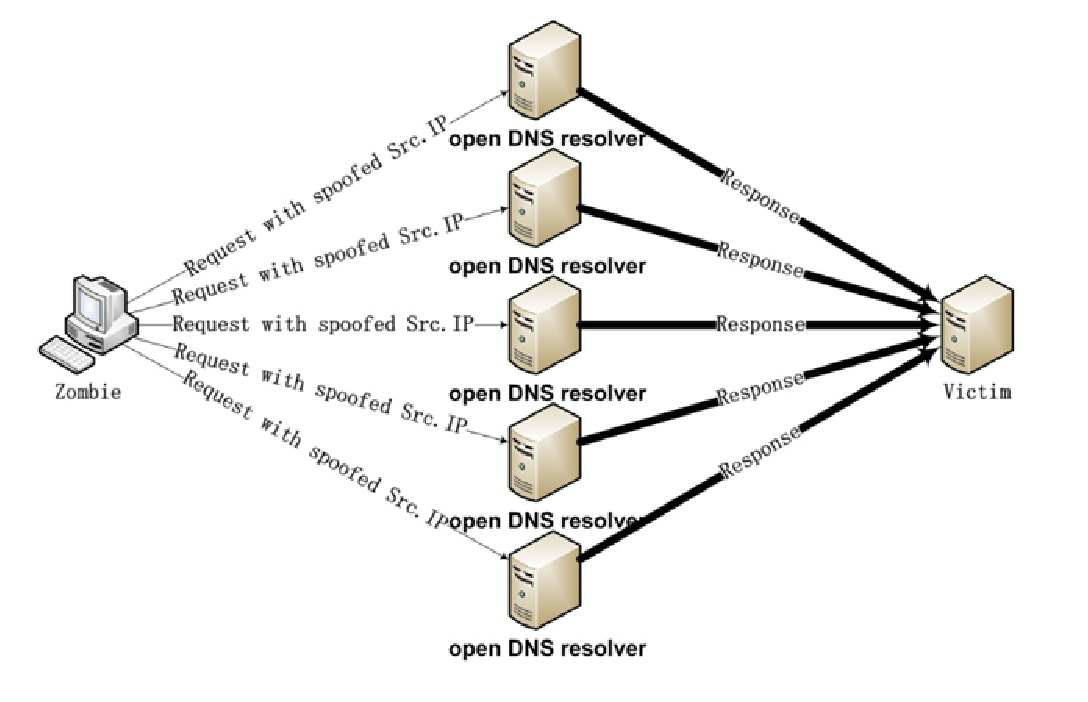
\includegraphics[width=\textwidth]{images/amplificationattacks}
\caption{Example of amplification attack with DNS}
\label{fig:amp_attack}
\end{figure}

For DTLS, the \texttt{ServerHello} is not larger than the \texttt{ClientHello} but amplification attack could still be possible (without the \texttt{HelloVerifyRequest}). Indeed, other messages are sent together with the \texttt{ServerHello}, including the one carrying the certificate (that could be quite large). Therefore, the additional step introduced with the \texttt{HelloVerifyRequest} (which is relatively small) prevents this kind of attack because the client has to prove it can answer at this address.

When the client sends its first \texttt{ClientHello}, the cookie field is initially empty. The server will then generate a new cookie which allows for a stateless exchange. It sends the \texttt{HelloVerifyRequest} with the cookie and doesn't remember anything about the client\footnote{This is indeed an exception to the retransmission measures. A \texttt{HelloVerifyRequest} will never be retransmitted, the client must first send another \texttt{ClientHello}.}. The DTLS server must generate cookies in such a way that they can be verified without retaining any per-client state on the server. A way to compute it is given in the RFC6347 section 4.2 \cite{rfc6347}:

\begin{lstlisting}
Cookie = HMAC(Secret, Client-IP, Client-Parameters)
\end{lstlisting}

The \texttt{Secret} is random and generated by the server. It could be periodically refreshed to invalidate previous cookies. Once a \texttt{ClientHello} has been received with a cookie, the server recomputes it and if both match, the connection can continue as in TLS with a \texttt{ServerHello} message.

\section{Typical DTLS communication}

\subsection{Handshake}

\begin{figure}[!h]
\centering
\begin{msc}[r]{DTLS Handshake}

\setlength{\instfootheight}{0em}
\setlength{\instheadheight}{0em}
\setlength{\instdist}{0.7\linewidth}
\setlength{\levelheight}{3em}

\declinst{client}{Client}{}
\declinst{server}{Server}{}

\mess{Client Hello}[t]{client}[0.3]{server}[1]
\nextlevel
\mess{Hello Verify Request}[t]{server}[0.3]{client}[1]
\nextlevel
\mess{Client Hello (w/ cookie)}[t]{client}[0.3]{server}[1]
\nextlevel
\mess{Server Hello}[t]{server}[0.5]{client}[1]
\nextlevel
\mess{Certificate}[t]{server}[0.5]{client}[1]
\nextlevel
\mess{Server Key Exchange}[t]{server}[0.5]{client}[1]
\nextlevel
\mess{Server Hello Done}[t]{server}[0.3]{client}[1]
\nextlevel
\mess{Client Key Exchange}[t]{client}[0.3]{server}[1]
\nextlevel
\mess{Change Cipher Spec}[t]{client}[0.3]{server}[1]
\nextlevel
\mess{Change Cipher Spec}[t]{server}[0.3]{client}[1]
\nextlevel
\nextlevel
\end{msc}
\caption{DTLS handshake with ECDHE-RSA cipher suite}
\label{fig:dtls-handshake}
\end{figure}


Figure \ref{fig:dtls-handshake} depicts a typical handshake with authentication of the server only and the ECDHE-RSA cipher suite\footnote{It means that Elliptic Curve Diffie-Hellman ephemeral is used for the key exchange and RSA for the signature.}. All messages before the \texttt{ChangeCipherSpec} are part of epoch 0. Their role is to negotiate the algorithms that will be used to compute the master key. The \texttt{Client Hello} has also the role to carry potential extensions supported by the client. If the server supports them as well, it will include them in the following \texttt{Server Hello} message. This is also where we chose to advertise our MPDTLS extension as explained in Chapter \ref{chap:design}.

The only difference with TLS (Section \ref{sec:tls}) is the presence of a second \texttt{ClientHello}. The first one is sent with no cookie and the second one must repeat the cookie received with the \texttt{HelloVerifyRequest}. Then the server confirms the cipher suite to be used through the \texttt{ServerHello} and directly sends its certificate and its ephemeral public key\footnote{In the case of ECDHE, it consists of the public DH parameters. Namely the domain parameters to define a particular curve.} including a signature of all previous exchanged messages. Finally the server sends the \texttt{ServerHelloDone} to explicitly say that the handshake is finished on its side.

Thereafter the client must also send its DH ephemeral public key. At this point, both parties have all the elements in their hands to compute the premaster secret. Note that unlike RSA, the secret is never communicated through the channel. With the random information exchanged through the \texttt{ClientHello} and \texttt{ServerHello}, each host can also compute the master key on its side. Consequently each peer will use this key to derive the set of keys used to communicate in the next epoch. The first messages of epoch 1 are the \texttt{ChangeCipherSpec} messages. They explicitly mark the separation between the handshake and the rest of the communication. Even if they are technically separated from the handshake, they are still considered as being part of it from a conceptual point of view.


\subsection{Application data}

Once the handshake has been completed, the peers can exchange Application Data packets. They are first encrypted and authenticated using the parameters negotiated earlier, then encapsulated into a Record Layer (Listing \ref{lst:dtls-record}).

DTLS doesn't bring any additional guarantee concerning the reliability of the link. As shown in Figure \ref{fig:dtls-data}, packets may be lost on the way and the application must deal with it. The sequence number for each message is indicated between chevrons. Sequence numbers are carried in clear inside the record layer, so each host knows how to verify the MAC and authenticate the packet.

\begin{figure}[!h]
\centering
\begin{msc}[r]{DTLS communication}

\setlength{\instfootheight}{0em}
\setlength{\instheadheight}{0em}
\setlength{\instdist}{0.7\linewidth}
\setlength{\levelheight}{3em}

\declinst{client}{Client}{}
\declinst{server}{Server}{}

\mess{Application Data <1>}[t]{client}[0.3]{server}[1]
\nextlevel
\mess{Application Data <1>}[t]{server}[0.3]{client}[1]
\nextlevel
\nextlevel
\lost[r]{Application Data<2>}[t]{}{client}[3]
\nextlevel
\mess{Application Data<3>}[t]{client}[0.3]{server}[1]
\nextlevel
\mess{Application Data<2>}[t]{server}[0.5]{client}[1]
\nextlevel
\nextlevel
\end{msc}
\caption{DTLS application data exchange}
\label{fig:dtls-data}
\end{figure}

\section{Use cases}

\label{sec:dtls-usage}

DTLS can be used almost everywhere UDP is used. We can think about applications such as VoIP (Voice over IP), multimedia, online gaming. Every application that wants to secure its communication but still benefit from faster transmission time of UDP may take advantage of using DTLS.

Of course the application has to cope with losses or reordering, but this is already the case for real time communication. As regards telephony, blank sounds replace the missing packets. For online gaming, high speed communication between the server and the client is needed to determine the character's position for instance. But if one packet is lost, the position can be determined by the next packet and the application will not be disturbed.

For video streaming applications, techniques are used to introduce a slight redundancy at the codec level in such a way that if some packets are lost, one frame may be missing but at least the video is still watchable\footnote{Of course, the application must a use a proper codec and compression method.}. It is also possible to introduce a small buffer to handle reordering.

In a recent Internet draft \cite{dtls-as-subtransport}, companies are trying to make DTLS the default sub-transport protocol for all application-level protocols when security is needed. This will raise DTLS to the rank of "good practice" for secured communications.

Another important use case for DTLS comes with its integration in WebRTC\footnote{\url{http://www.webrtc.org/}}. This is an open project which has an objective to bring real time communications to browsers and mobile applications via simple APIs. In this context, DTLS has been chosen to ensure the communication between two peers (i.e. browsers or mobile apps). The internet draft describing the security architecture of WebRTC \cite{ietf-rtcweb-security-arch} proposes to use SRTP over DTLS for multimedia communications and DTLS alone for any other kind of data. Figure \ref{fig:webrtc} is taken from a presentation \cite{rescorla2011proposed} made by E.Rescorla and shows how the connection is set up in this proposed design.  

\begin{figure}[!ht]
\centering
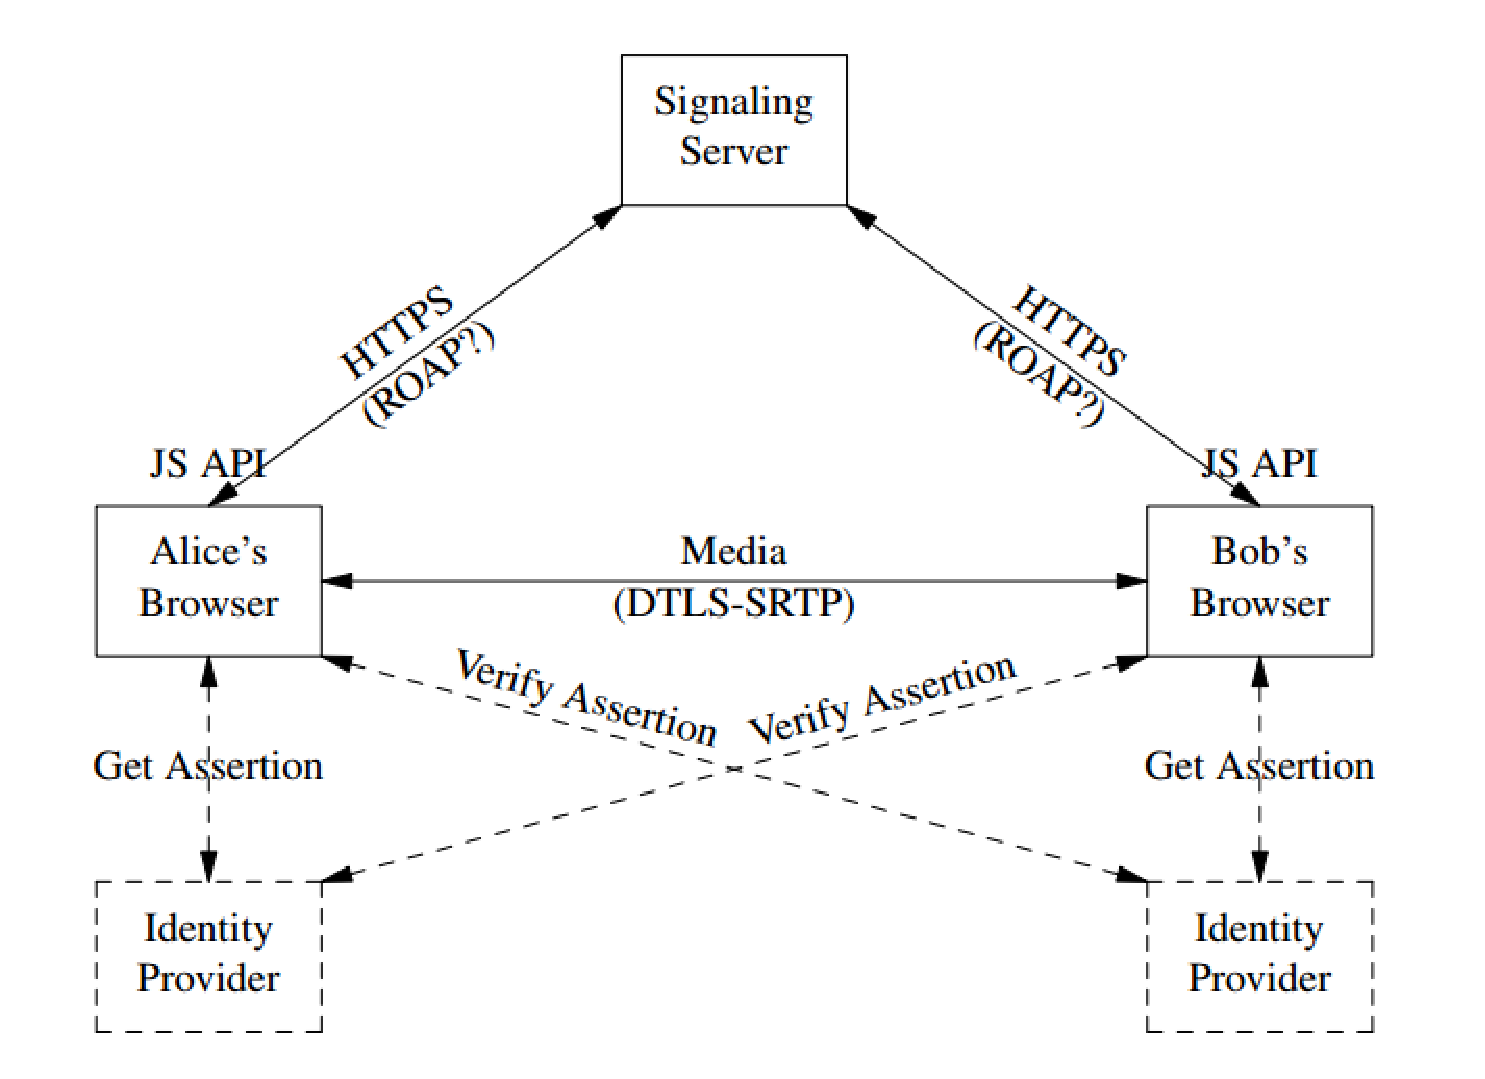
\includegraphics[width=0.9\textwidth]{images/webrtc.eps}
\caption{Proposed design for WebRTC security architecture}
\label{fig:webrtc}
\end{figure}

By the peer to peer nature of this application, a signalling server is needed to act as a "rendez-vous" point and to perform NAT traversal. Then the handshake can take place and identity providers issue and verify certificates. Finally all data are transmitted through the DTLS transmission and multiple SRTP sessions can use the same DTLS session. 

To sum up, all these applications may benefit from using DTLS but also MPDTLS as it will allow more resilience and better performances. We will demonstrate this point in the following chapters.

\section{Security considerations}
\label{sec:tls-sec}

Most of the security considerations are the same as those of TLS 1.2 \cite{RFC5246} since DTLS is only an adaptation of TLS for unreliable transport protocols.

The attacks known for TLS could theoretically be used for DTLS as well. This is the case for the "secure renegotiation". As a reminder, this vulnerability allows an attacker who can hijack a HTTPS connection to add custom request to a communication between the client and the web server. Even if the attacker cannot retrieve the content of the communication, it can still have dramatic consequences. As depicted on Figure \ref{fig:tls-reneg} taken from \cite{tls-reneg}, an attacker can inject bank orders and then trigger the renegotiation with a real client. The bank order is only delayed and when the renegotiation is completed, it is executed before anything else. The best solution up to know is to disable by default this feature on servers. \todo{Or to implement the extension RFC5746}

\begin{figure}[!ht]
\centering
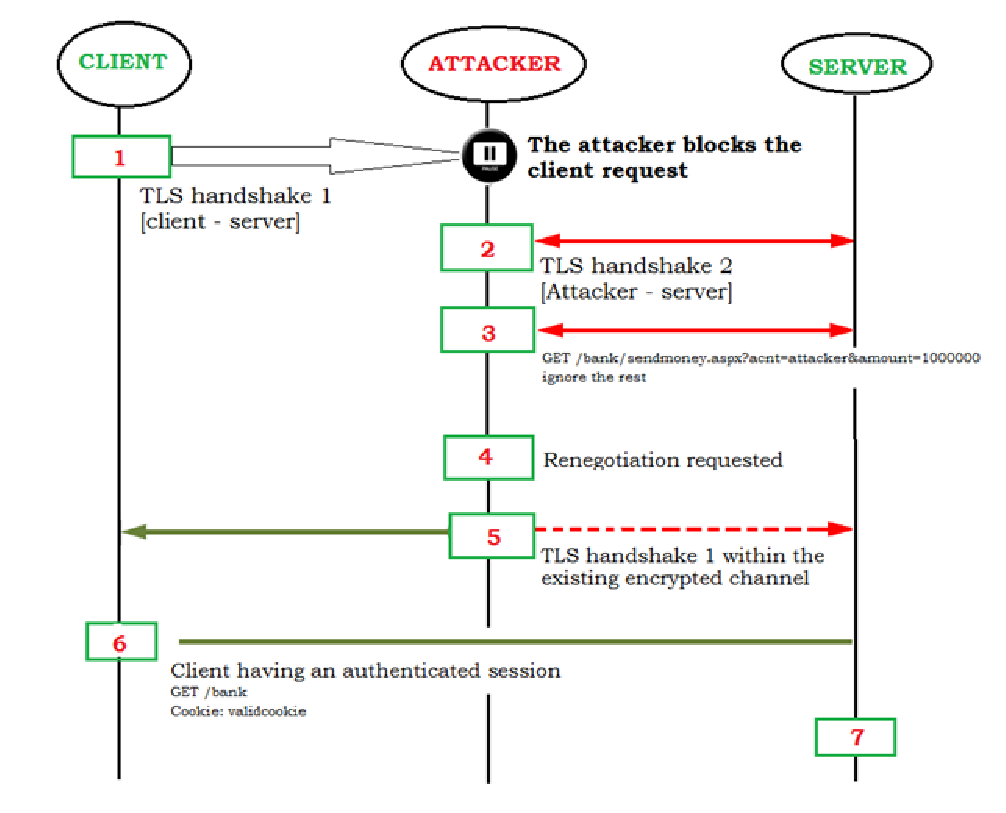
\includegraphics[width=0.8\textwidth]{images/TLSrenegotiation}
\caption{TLS renegotiation vulnerability}
\label{fig:tls-reneg}
\end{figure}

Other attacks could also be applied to DTLS and be more efficient on DTLS than on TLS, namely the DoS attacks. Two main categories can be identified :

\begin{itemize}
\item The blind DoS : packets are being transmitted with a spoofed IP address to redirect the traffic to another target (amplification attack) or to simply not diclose the IP address of the attacker. They are called blind because the attacker will never receive any answer from the server. They are made easier with UDP because no handshake is needed with the server.
\item Computational DoS : the attacker can reply to certain messages but will try to optimize the ratio between the work he has to do and the work he is asking to the server.
\end{itemize}

Blind DoS are made impossible in TLS because the attacker must first complete the TCP handshake and thus prove he can answer at this address. As presented earlier, the introduction of the \texttt{Hello Verify Request} will prevent this kind of attack for DTLS too.  Although it is not a strict requirement to implement this feature in DTLS (\cite{rfc6347} Section 5), it is strongly recommended for DTLS servers  unless there is a good reason to think that no amplification is possible in their environment.

Nevertheless the second type can still be used to disturb a server running DTLS or even TLS. As explained by E. Rescorla in \cite{tls-dos}, nothing is done at the design level to prevent these kind of attacks because it would imply putting a lot of work on the client side. It is generally a bad idea for performances. Moreover, the attackers are often using infected computers of casual people to launch DoS attacks. Therefore they have a lot of CPU power available anyway.

\section{Heartbeat extension}

The heartbeat extension is unfortunately known for the famous heartbleed bug\footnote{\url{http://heartbleed.com/}} detected in April 2014. Every server using OpenSSL at this time was vulnerable and part of the memory could be retrieved (including private keys, passwords\dots). It is important to note that the error came from the implementation of the extension inside OpenSSL and not from the standard itself.

Anyway, this extension can be really useful to assess the availability of a link and also provides a keep-alive feature. It is quite simple but it also allows for extensibility and new messages as stated in RFC6520 \cite{rfc6520}. The structure of a heartbeat message is presented on Listing \ref{lst:hb-msg}. This will take place on top of the Record Layer (Listing \ref{lst:dtls-record}). The advertisement of this extension is made through a Hello extension. It also defines the behavior of the hosts upon the reception of Heartbeat messages.

\addtypes{HeartbeatMessageType}
\begin{lstlisting}[caption=Heartbeat message, label=lst:hb-msg]
struct {
  HeartbeatMessageType type;
  uint16 payload_length;
  opaque payload[HeartbeatMessage.payload_length];
  opaque padding[padding_length];
} HeartbeatMessage;
\end{lstlisting}

For now, only two types of Heartbeat messages are in use : \texttt{Heartbeat Request} and \texttt{Heartbeat Response}. The response must contain the same payload as the one in the request triggering it. A simple exchange is presented on Figure \ref{fig:heartbeat}.

\begin{figure}[!h]
\centering
\begin{msc}[r]{Heartbeat request/response}

\setlength{\instfootheight}{0em}
\setlength{\instheadheight}{0em}
\setlength{\instdist}{0.7\linewidth}
\setlength{\levelheight}{3em}

\declinst{host1}{Host 1}{}
\declinst{host2}{Host 2}{}

\lost[r]{Heartbeat Request}[t]{}{host1}[3]
\nextlevel
\mess{Heartbeat Request}[t]{host1}[0.3]{host2}[1]
\nextlevel
\mess{Heartbeat Response}[t]{host2}[0.5]{host1}[1]
\nextlevel
\nextlevel
\end{msc}
\caption{Heartbeat requests and responses}
\label{fig:heartbeat}
\end{figure}

Other messages may be implemented since a new IANA section has been opened to register the different \texttt{HeartbeatMessageType}. Indeed, as you will see in the Chapter \ref{chap:implementation}, we have designed a new type of message used to transmit a timestamp.

\chapter{Implementation}\label{chap:implementation}

Since we designed MPDTLS as an extension for DTLS, it was logical to not implement it from scratch but start from an existing implementation of DTLS. Multiple libraries implement the latest version \footnote{\url{https://en.wikipedia.org/wiki/Datagram_Transport_Layer_Security\#Implementations}}, but we choose wolfSSL \cite{wolfssl} (previously CyaSSL) as our starting point.

The choice was done following multiple criteria :

\begin{itemize}
\item Clarity of code
\item Documentation
\item Existing examples
\item Library size
\end{itemize}

Unlike OpenSSL, wolfSSL contains a reduced number of files to handle SSL/TLS and DTLS. The objective of this library is to be as light as possible to allow integration in embedded systems. As stated in their official website \footnote{\url{http://www.yassl.com/yaSSL/Home.html}}, the library is up to 20 times smaller than OpenSSL.

A documentation and working examples are provided to help people using it. For all these reasons, we chose to go with wolfSSL. In the following sections, we are going to explain how this library works, how we integrate our additions to DTLS and the various problems we had to face during the implementation.

\section{Packet reception}
The first step is to make the library recognizes the new packets and handles them correctly, like issuing a \texttt{FeedbackAck} upon reception of a \texttt{Feedback}. This part is quite easy once the internal flow followed by the received packets is understood. The flow we are going to explain is pictured in the Figure \ref{fig:readdiag}. The call related to mutex are not part of the original wolfSSL code and are explained in the Section \ref{sec:threadsafe}.

First of all, it is important to recall wolfSSL is a library and thus does not have any existence outside the call made in the client code.

To receive packets, an application must call the \texttt{wolfSSL\_read(WOLFSSL*,void*,int)} function once all the library is correctly set up. When this function is call, the process enters the library, dives into the \texttt{ReceiveData} and \texttt{ProcessReply} functions and will eventually make a blocking call into the \texttt{CBIORecv} macro\footnote{The low-level mechanisms to read and write on sockets are indeed encapsulated into macros selected following the compilation or configuration flags. This provides to the library some cross-platform aspects.} to listen on the socket. When a new packet arrives, the process is woke up and it copies the packet into an internal buffer. Once the copy is made and the pointers correctly set, the process can treat the packet.

\begin{figure}[!h]
\centering
\begin{sequencediagram}
\centering
\newthread[blue]{r}{wolfSSL\_read}
\newinst{rd}{ReceiveData}
\newinst{pr}{ProcessReply}
\newinst{gid}{GetInputData}
\newinst{rc}{Receive}
\newinst{grh}{GetRecordHeader}
%\newinst{do}{Do\textit{Type}}

\begin{call}{r}{MutexLock}{r}{}
\end{call}
\begin{call}{r}{}{rd}{}
    \begin{sdblock}{while}{no content in \texttt{clearOutputBuffer}}
        \begin{call}{rd}{}{pr}{}
            \begin{call}{pr}{}{gid}{}
                \begin{call}{gid}{}{rc}{}
                    \begin{call}{rc}{MutexUnlock}{rc}{}
                    \end{call}
                    \begin{call}{rc}{\texttt{CBIORecv}}{rc}{}
                        \postlevel
                    \end{call}
                    \begin{call}{rc}{MutexLock}{rc}{}
                    \end{call}
                \end{call}
            \end{call}
            \begin{call}{pr}{}{grh}{\shortstack{\textit{ContentType}\\Length}}
                \postlevel
            \end{call}
            \begin{sdblock}{switch}{on \textit{ContentType}}
                \begin{call}{pr}{Do\textit{ContentType}}{pr}{}
                    \postlevel
                \end{call}
            \end{sdblock}
        \end{call}
    \end{sdblock}
\end{call}
\begin{call}{r}{MutexUnlock}{r}{}
\end{call}
\end{sequencediagram}
\caption{Major functions called on \texttt{wolfSSL\_read()}\label{fig:readdiag}}
\end{figure}


First, it reads the RecordLayer header, containing the length of the packet and the type of the Record. The latter can be one of the \texttt{ContentType} value defined in the RFC. During this verification, it also define, based on the \texttt{ContentType} value, if the packet is encrypted and therefore needs to be deciphered before handling it.

Then, after the decryption of the packet if it was needed, the packet is dispatched to the handling function corresponding to the Record type. These functions are called following the pattern "\texttt{Do}\textit{TypeName}" (e.g. \textit{DoApplicationData} to handle AppData packets). For the sake of clarity, these two steps (decryption and all possible \texttt{Do}functions) are not represented on the Figure \ref{fig:readdiag}.


In the case of the original implementation of wolfSSL, the only Record type that could be encountered at this point was AppData. The function \textit{DoApplicationData} does some treatments on the packet like verifying the MAC or decompressing the packet if needed and finally copies the clear content of the packet into a specific buffer called \texttt{clearOutputBuffer}. Then, if the input buffer has been completely consumed, the process comes back to the function \texttt{ReceiveData}. This function copies the content of \texttt{clearOutputBuffer} to the application buffer passed in argument of \texttt{wolfSSL\_read}, giving to the client application the content of the received packet. The library will then exit and give the control back to the calling code.

\subsection{Adding new types}

Adding the recognition of a new type is done in two steps, after the defininion of all the needed declarations in the header file: we start by adding the type in the switch of the \texttt{GetRecordHeader} function. We can also add indication about the packet type, such as if the content is ciphered or not. Then, we need to add a new case for the type in the switch statement of the \texttt{ProcessReply} function, in which we prepare and make the call to a new, dedicated function \texttt{Do\textit{TypeName}}.

Now that library recognizes the new type and call the appropriate \texttt{Do}function, we can implement the latter with the intended behavior. In our case, we use the \texttt{DoApplicationData} as a base for the implementation of all the \textit{Do}function of protocol-level packet types (e.g. \texttt{Feedback}, \texttt{WantConnect}\dots). It is the easiest solution to get ciphering and authentication of the packets.But it is important to not let these packets leave the library and be delivered to the application. To achieve this, we move the pointer marking the end of the \texttt{clearOutputBuffer} before the beginning of the current packet, once we have finished the treatment of the packet.

\section{Packet emission}

The packets emission is even simpler, as we don't have to wait for some event, we trigger it. So, in wolfSSL, an application can send packets by the use of the \texttt{wolfSSL\_write(WOLFSSL*, void*, int)} function. As shown in the Figure \ref{fig:writediag}, the process then enters in \texttt{SendData}, which is responsible of all the authentication and encryption stuff, in the original code of the library. We moved the code handling the MAC and encryption in a new function \texttt{SendPacket}, allowing us to use the encryption not only for the Application Data packets but also for our protocol-level packets. As for the receiving functions, we created a set of \texttt{Send\textit{TypeName}} functions, in charge of building the corresponding packets before sending them. All these methods end by calling \texttt{SendPacket} which will then call \texttt{SendBuffered}. \texttt{SendBuffered} is the last function in the library before leaving the control to the concrete sending macro \texttt{CBIOSend}, and this is the place we choose to put our scheduling mechanism. The socket to use is thus chosen at the beginning of \texttt{SendBuffered}, just before the call to the sending function.

\begin{figure}[!h]
\centering
\begin{sequencediagram}
\centering
\newthread[blue]{w}{wolfSSL\_write}
\newinst{sd}{SendData}
\newinst{sp}{SendPacket}
\newinst{bm}{BuildMessage}
\newinst{sb}{SendBuffered}
%\newinst{do}{Do\textit{Type}}

\begin{call}{w}{MutexLock}{w}{}
\end{call}
\begin{call}{w}{}{sd}{}
        \begin{call}{sd}{}{sp}{}
            \begin{call}{sp}{}{bm}{}
                \begin{call}{bm}{AddRecordHeader}{bm}{}
                    \postlevel
                \end{call}
                \begin{call}{bm}{Encrypt}{bm}{}
                    \postlevel
                \end{call}
                \begin{call}{bm}{HashOutput}{bm}{}
                    \postlevel
                \end{call}
            \end{call}
            \begin{call}{sp}{}{sb}{}
                \begin{call}{sb}{\texttt{CBIOSend}}{sb}{}
                    \postlevel
                \end{call}
            \end{call}
        \end{call}
\end{call}
\begin{call}{w}{MutexUnlock}{w}{}
\end{call}
\end{sequencediagram}
\caption{Major functions called on \texttt{wolfSSL\_write()}\label{fig:writediag}}
\end{figure}

\section{Thread-safety}\label{sec:threadsafe}

A major drawback of living at the application-level as a library is that you are really dependent of the application that uses you. For instance, all protocol-level packets need responses to ensure the reception, since DTLS is not reliable. But, to trigger the internal mechanisms explained in the previous sections, the library must be in a listening state, constantly. If an application needs to send some packets, which seems to be a normal use case of the library, it will need to use threads to read and write simultaneously. For this reason, we need to be sure that using the library in such way will not cause trouble. As the library uses a lot of internal buffers when it reads or writes, and that our treatments of protocol-level packets involves packets emission during packets reading, we considered the whole library code as a critical section, with a notable exception for the blocking call in the \texttt{Receive} function\footnote{As a call to \texttt{select} is blocking, it prevents the application to write packets when the other thread waits for incoming packets, which would add an extra undesirable overhead.}.

Thus, as with every critical section that you want to protect, we added a mutex to lock when entering either \texttt{wolfSSL\_read} or \texttt{wolfSSL\_write} and unlocked just before leaving these functions. This mutex is also unlock just before the blocking call to select and relock right after the select returns.

\subsection{What about processes ?}

Using processes instead of the threads is another solution, but either processes have to use different session credentials or have to share memory to use the same session object. One could propose to simply duplicate the session either through the session resuming or via copy-on-write session mechanisms, but just having the same session credentials is not sufficient to the library to correctly work. As we use statistics to choose the best path to send new packets, the session object must be completely in sync between the processes, with all the risks of memory corruption due to the simultaneous accesses. We finally end up in the same situation as with the threads.

For the sake of simplicity, we recommend thus to simply use threads, as we made our best to get a thread-safe library.

\section{Managing retransmissions}

\subsection{Timeouts}

\subsection{Packets count}

\section{Multipath integration}
\subsection{}

%\chapter{Performance Evaluation}\label{chap:perfs}

\section{Test application}\label{sec:vpnapp}

As MPDTLS is implemented inside a library, we need an application to use it. We tried to find out an existing application that could be a good candidate for our tests. First, we needed an application which uses DTLS for most of its communications. It was surprisingly hard to find but we still managed to find one : Campagnol\cite{campagnol}. Campagnol is a decentralized VPN solution that uses DTLS to communicate between the peers. Unfortunately, for reasons exposed in Appendix \ref{app:campagnol}, we were unable to integrate correctly our modified library within this application.

So, we took the decision to build a simple VPN application \cite{mpdtls-vpn} by reusing some part of Campagnol code. A VPN application is indeed perfectly suitable for all the experiences we could imagine : potentially any application can use a VPN tunnel without even noticing it. Each packet is encapsulated inside a DTLS packet transmitted securely between the two MPDTLS hosts (see Figure \ref{fig:vpn}).

\begin{figure}[!ht]
\centering
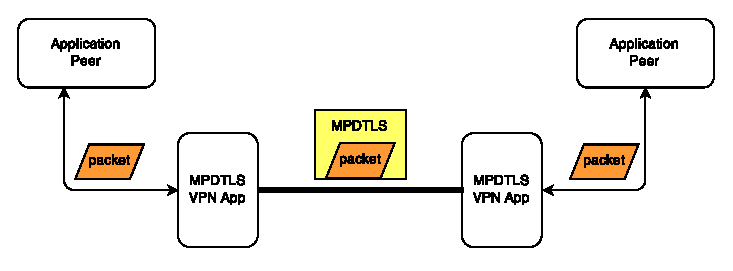
\includegraphics{images/vpn.eps}
\caption{A simple VPN application using MPDTLS}
\label{fig:vpn}
\end{figure}

The behavior of such a MPDTLS VPN App is shown on Figure \ref{fig:vpn-io}. A TUN interface is created with a specified address and netmask. Every packet going to an address falling in this netmask is sent by the kernel to this interface. Then we need to monitor this interface, to read the incoming packets and to sent them through the tunnel. This is the job of the first thread (in red on the Figure). We also need to capture packets coming from the network and to forward them to the TUN interface. This is handled by a second thread represented in green on the Figure. Finally, a last thread (in blue) listens to the standard input for potential commands. This is the channel that we use to communicate with the application to add or remove new interfaces for instance. We can ask for debug information or even change the scheduler policy on the fly.

\begin{figure}[!ht]
\centering
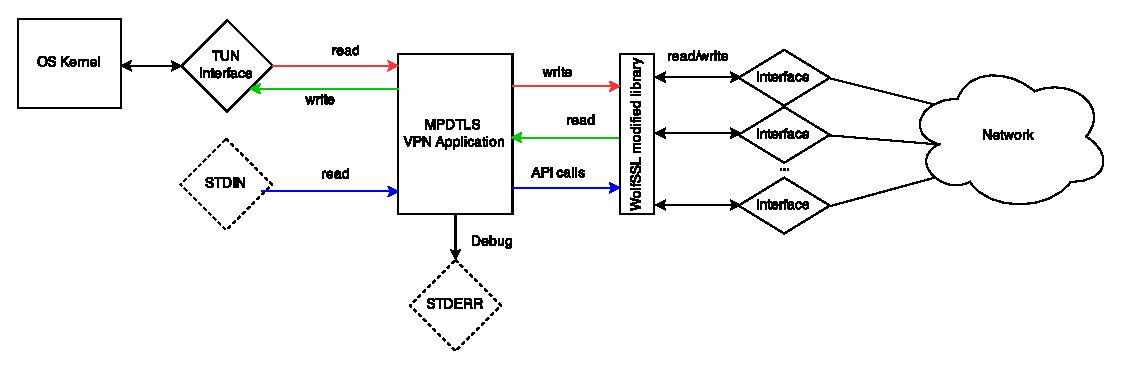
\includegraphics[width=\textwidth]{images/tunneling-IO.eps}
\caption[I/O interactions for one host of our application]{I/O interactions for one host of our application. Each thread is represented with one color.} 
\label{fig:vpn-io}
\end{figure}

One of the most useful information we can ask for are the statistics for a particular flow. Looking at this output, we can identify most of the time an issue without analyzing at the packet trace. An example of such an output is shown on Listing \ref{lst:stats}. We can easily see the part of the traffic that the subflow is actually supporting, the estimated delays and other information. The separator "|" used in the \texttt{packets sent} list differentiates the ones that are in the waiting status and the others (see Section \ref{sec:impl-stats} for more details about this waiting status).

\begin{lstlisting}[language=bash,caption=An output of the statistics for a particular flow,label=lst:stats]
---- Stats Flow N 0 ---- 
IP src : 11.0.0.1 
IP dst : 11.2.0.1 
Support 41 % of the connection
----- Receiver Stats ----- 
Packets received : 44 
Min_Seq received : 76 
Max_Seq received : 172 
Backward delay : 10 ms
----- Receiver Cache ----- 
Packets received : 0 
Min_Seq received : 2147483647 
Max_Seq received : 0 
----- Sender Stats ----- 
Packets sent : [ 8487 8489 8492 ... 8633 8634 8636 | 8640 8642 ... 8706 8707] 
Forward delay : 10 ms
Loss Rate : 0.000000 
---------------------------

\end{lstlisting}

\section{Different scheduler policies}\label{sec:perf-sched}

We present here three examples of scheduler strategies that we have implemented and how the fractional distribution is computed in each case. As conclusion, each of them has pros and cons. The good choice is strongly related with what the underlying application expects to do. In some cases, an application could want to build its own scheduler and this matches with our design since we provide a dedicated customisable callback.


\subsection{\texttt{Round Robin}}

The round robin is the simplest strategy consisting in sending the same amount of packets over each available link. This does not use any of the information gathered from the feedback. However it may be a good choice if we know in advance that the different links share common properties (e.g. in a datacenter).

The fractional distribution is really easy to compute as every link will get the same fraction of the traffic (in terms of number of packets).

\begin{equation*}
f_i = \frac{1}{n}
\end{equation*}

where $f_i$ is the portion of traffic given to flow $i$ and $n$ is the total number of subflows.

\subsection{\texttt{Optimize Latency}}

For this strategy, we want to give more weight to the links where the forward delay is lower. We have to keep in mind that every delay $d_i$ contains the clock desynchronization term $\Delta T$ (see Section \ref{sec:forward-delay}). In order to get rid of this term, we must consider the difference with another delay. We choose to take the difference with the maximum delay as by definition the greater the difference, the smaller the delay. This maximum will evolve and is defined as the maximum delay reported on every flow at the time we compute this fractional distribution. Equation \ref{eq:latency} gives the complete expression.  

\begin{equation}
f_i = \frac{max_d - d_i + \alpha}{\sum_j (max_d - d_j) + n*\alpha }\quad \text{where } \quad max_d = max_i(d_i) 
\label{eq:latency}
\end{equation}

Without the $\alpha$ term, the flow with the maximum delay will never be used. Indeed if you have two subflows with forward delays of 10ms and 20ms and $\alpha=0$, then $100\%$ of the traffic will be supported by the first subflow. Although this could appear as an optimal choice, it is always preferable to send a small part of the traffic on each link just to monitor the characteristics and to keep receiving feedback and heartbeat messages. After some tests, we think the value of $\alpha$ must be defined between 5\% and 10\% of $max_d$\footnote{Of course, $max_d$ must not be null. If it is the case, then a constant value must be chosen like 1ms and the equation will actually give the same result as a round robin.} to give the best results. 

\subsection{\texttt{Optimize Loss}}

Another strategy that we could consider is to favor the less congested links. In this case, we give more priority to a link with the smallest loss rate. The principle is almost the same as for the latency, we consider the difference with the biggest loss rate observed. The idea is to quantify the relative differences between the subflows.

We may be tempted to use directly the loss rate reported in the statistics. However if the link experiences severe losses, we may not be aware of it because all the feedback packets have been dropped. Therefore we compute what we call the "real" loss rate which also takes in consideration the number of packets sent and not yet acknowledged. Equation \ref{eq:lr} gives the formula used and $feedback_{thr}$ is the number of packets after which we send a feedback. We consider two times this amount to give a penalty to the link because after one feedback, packets are in waiting status and need another feedback before being completely forgotten. The penalty $pen$ is computed as two times the probability of loosing one feedback. The factor $2$ here will probably need some tuning but the idea is to boost the penalty as the risk is rather small to loose only the feedback packet but no application data. 

\begin{align}
LR_i &= stats_{LR} + \left \lfloor{\frac{pckts_{sent}}{2 * feedback_{thr}}} \right \rfloor  * pen & \text{where } \quad pen = \frac{1}{feedback_{thr}} * 2 \label{eq:lr} \\
f_i &= \frac{max_{LR} - LR_i + \beta}{\sum_j (max_{LR} - LR_j) + n*\beta } & \text{where } \quad max_{LR} = max_i(LR_i) 
\label{eq:losses}
\end{align}

Equation \ref{eq:losses} is really similar to Equation \ref{eq:latency} and we also need a constant term $\beta$ for the same reasons. After some tests, we arrive at the conclusion that a suitable value for $\beta$ is around $1\%$  of the loss rate in most situations.

\section{Multipath simulations}

We have designed an environment to evaluate our system under different conditions. All the following measures take place inside a Mininet laboratory \cite{mininet} to easily set up the topology we want and to create multiple interfaces. Also, we used a kind of framework for Mininet called Minitopo\cite{minitopo} to easily configure the topology and create automated tests just with configuration files instead of scripts. To generate network traffic, we used the D-ITG (Distributed Internet Traffic Generator)\cite{ditg} tool. More details about how to reproduce these graphs and the following are given in Appendix \ref{app:graph}.

\subsection{Topology}\label{sec:perftopo}

The topology used for the following evaluations is the one presented on Figure \ref{fig:topo-phys}. We have four interfaces on the client side that are linked to a network router and one link between the router and the server. Note that the latter is not constrained, we will only change the characteristics of the first 3 paths shown on the Figure. The path 4 is reserved for the signaling of D-ITG to avoid any interference with our measures.


\begin{figure}[!ht]
\centering
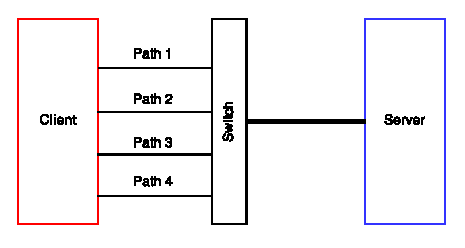
\includegraphics[width=0.7\textwidth]{images/perf-topo-phys.eps}
\caption{Physical topology inside mininet}
\label{fig:topo-phys}
\end{figure}

The corresponding logical topology is depicted on Figure \ref{fig:topo-log}. We are using 3 flows concurrently between the client and the server. The D-ITG application is sending traffic to one unique TUN interface and the traffic goes through our tunnel to reach the D-ITG receiver.

\begin{figure}[!ht]
\centering
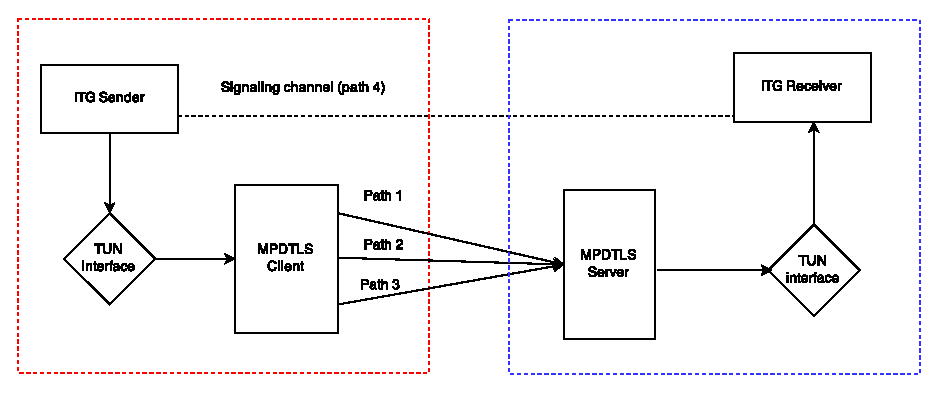
\includegraphics[width=\textwidth]{images/perf-topo-logic.eps}
\caption{Logical topology used for measurements}
\label{fig:topo-log}
\end{figure}

\subsection{Traffic balancing}

The first thing to evaluate is if we really take advantage of multiple interfaces and how we balance the traffic between them. We performed experiments to determine in which conditions each scheduler works well and how they compute the distribution of traffic in various environments.

\subsubsection{With dynamic bandwidth}

In this experiment, we have tested the two schedulers that are taking the context into consideration : \texttt{Optimize Latency} and \texttt{Optimize Loss}. The configuration used is the following (the path indexes refer to Figure \ref{fig:topo-log}) :


\begin{center}
\begin{tabular}{|c|c|c|c|}
\hline
Path n\degree & bandwidth & loss rate & delay  \\ \hline
1 &  1 Mbps & 0 & 10ms \\ \hline
2 & variable & 0 & 20ms \\ \hline
3 & not used & - & - \\ \hline
\end{tabular}
\end{center}

We ran the experiment with multiple values of bandwidth of path 2 to see how its usage rate is impacted. We have generated constant traffic with D-ITG \cite{ditg} using both UDP and TCP. All these results are reported in Figure \ref{fig:dynbw}. The measurements have been obtained with sessions of 60 seconds and every experiment has been repeated 11 times to evaluate the mean. The 95\% confidence interval of the mean is presented in white and has been computed with a Student T distribution.


\begin{figure}[!ht]
\centering
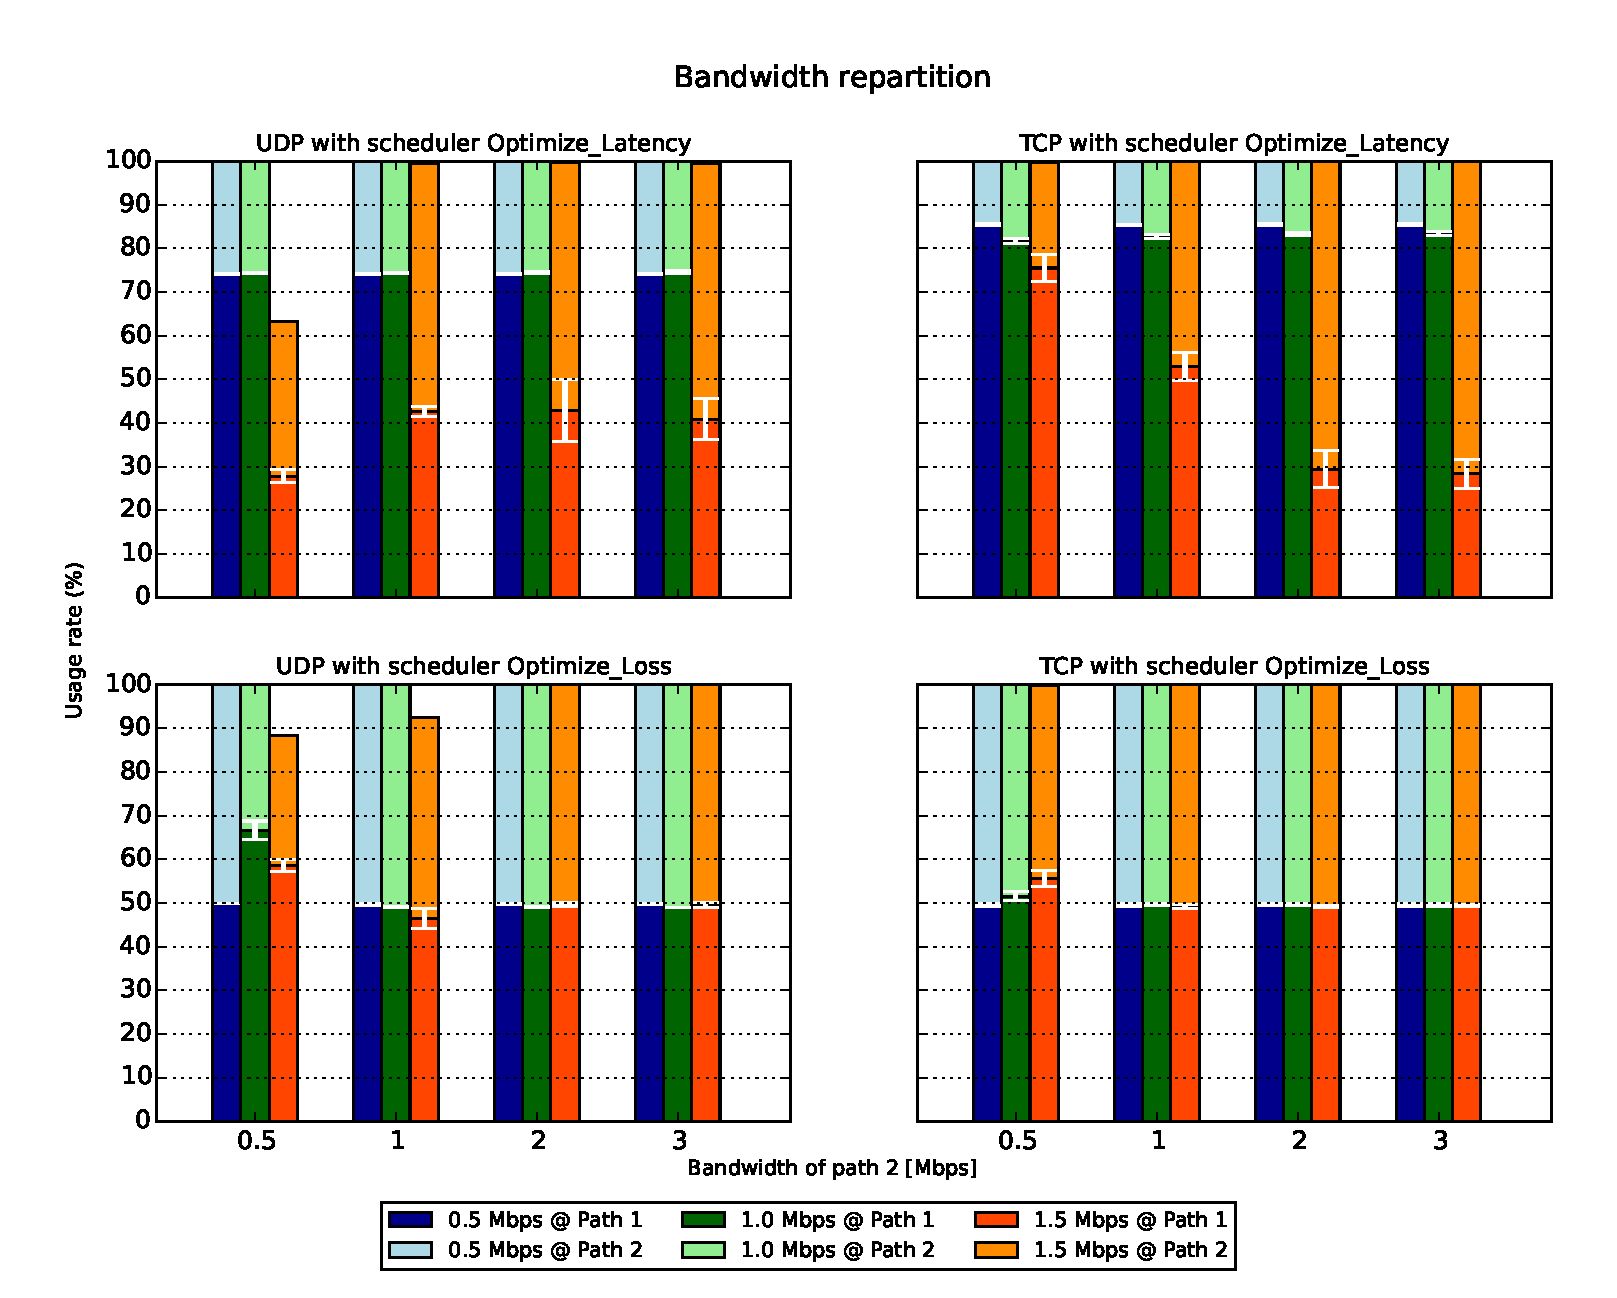
\includegraphics[width=\textwidth]{images/xp/graph1.eps}
\caption{Usage repartition with bandwidth variation}
\label{fig:dynbw}
\end{figure}


For every bandwidth value of path 2, we have 3 bars that represent the total traffic we are trying to send through the tunnel. Each bar is separated in two parts that show the amount of traffic passing through each path in bytes/sec. The losses are easily identifiable because they occur every time the total usage does not reach the total bandwidth. Of course at the beginning we have congestion because if path 2 can support only $0.5Mbps$ then $bw(p1) + bw(p2) = 1.5Mbps$ and in the last case we are trying to send traffic at 1.5Mbps. So, it is supposed to use 100\% of the tunnel capacity which is impossible in practice. Moreover, this computation does not even take into account the overhead introduced by the encapsulation inside DTLS. Indeed, we are sending packets of size 825 bytes into the TUN interface and the resulting size of the DTLS \texttt{ApplicationData} packet is 905 bytes; so an overhead of 80 bytes (almost 10\% in this case).

First, it is interesting to confirm that the \texttt{Optimize loss} scheduler performs better if we are dealing with congested links and especially with UDP. Note that TCP doesn't experience losses in the same way as UDP because it will reduce its transmission rate internally with the congestion window mechanism. So even if we impose a given volume of traffic, the real bandwidth will be lower with TCP in case of congestion.

Secondly, we observe an unexpected phenomenon if we look at the graph "UDP with scheduler Optimize Latency" : when we increase the total bandwidth to 1.5Mbps (orange), it does not optimize latency at all. Indeed, it gives only a small part of the traffic to the faster link. We have tracked down the problem and it is apparently coming from a bad perception of the forward delay. At the beginning, it uses extensively path 1 as expected but rapidly reaches congestion as the capacity of path 1 is 1Mbps. The heartbeat messages that are used to evaluate the forward delay are themselves postponed by a few milliseconds due to this congestion and it is sufficient for the scheduler to estimate the delay is better on path 2. Even if the forward delay is later correctly estimated, we go back in the same cycle.  It is not the case with TCP at least at the beginning because TCP reduces the bandwidth to fit into the tunnel and therefore there is no congestion observed.

\subsubsection{With dynamic loss rate}\label{sec:perfs-loss}

This time, we want to see how the schedulers react with various loss rate at one of the paths. The configuration is the following :

\begin{table}[!ht]
\centering
\begin{tabular}{|c|c|c|c|}
\hline
Path n\degree & bandwidth & loss rate & delay  \\ \hline
1 &  1 Mbps & 0 & 10ms \\ \hline
2 & 3 Mbps & variable & 10ms \\ \hline
3 & not used & - & - \\ \hline
\end{tabular}
\end{table}

Again we are using 2 paths only and they have the same latency but different bandwidths. We run different experiments with 4 values of loss rate for path 2, going from 0\% to 3\%. The results we have obtained are presented on Figure \ref{fig:dynloss}.


\begin{figure}[!ht]
\centering
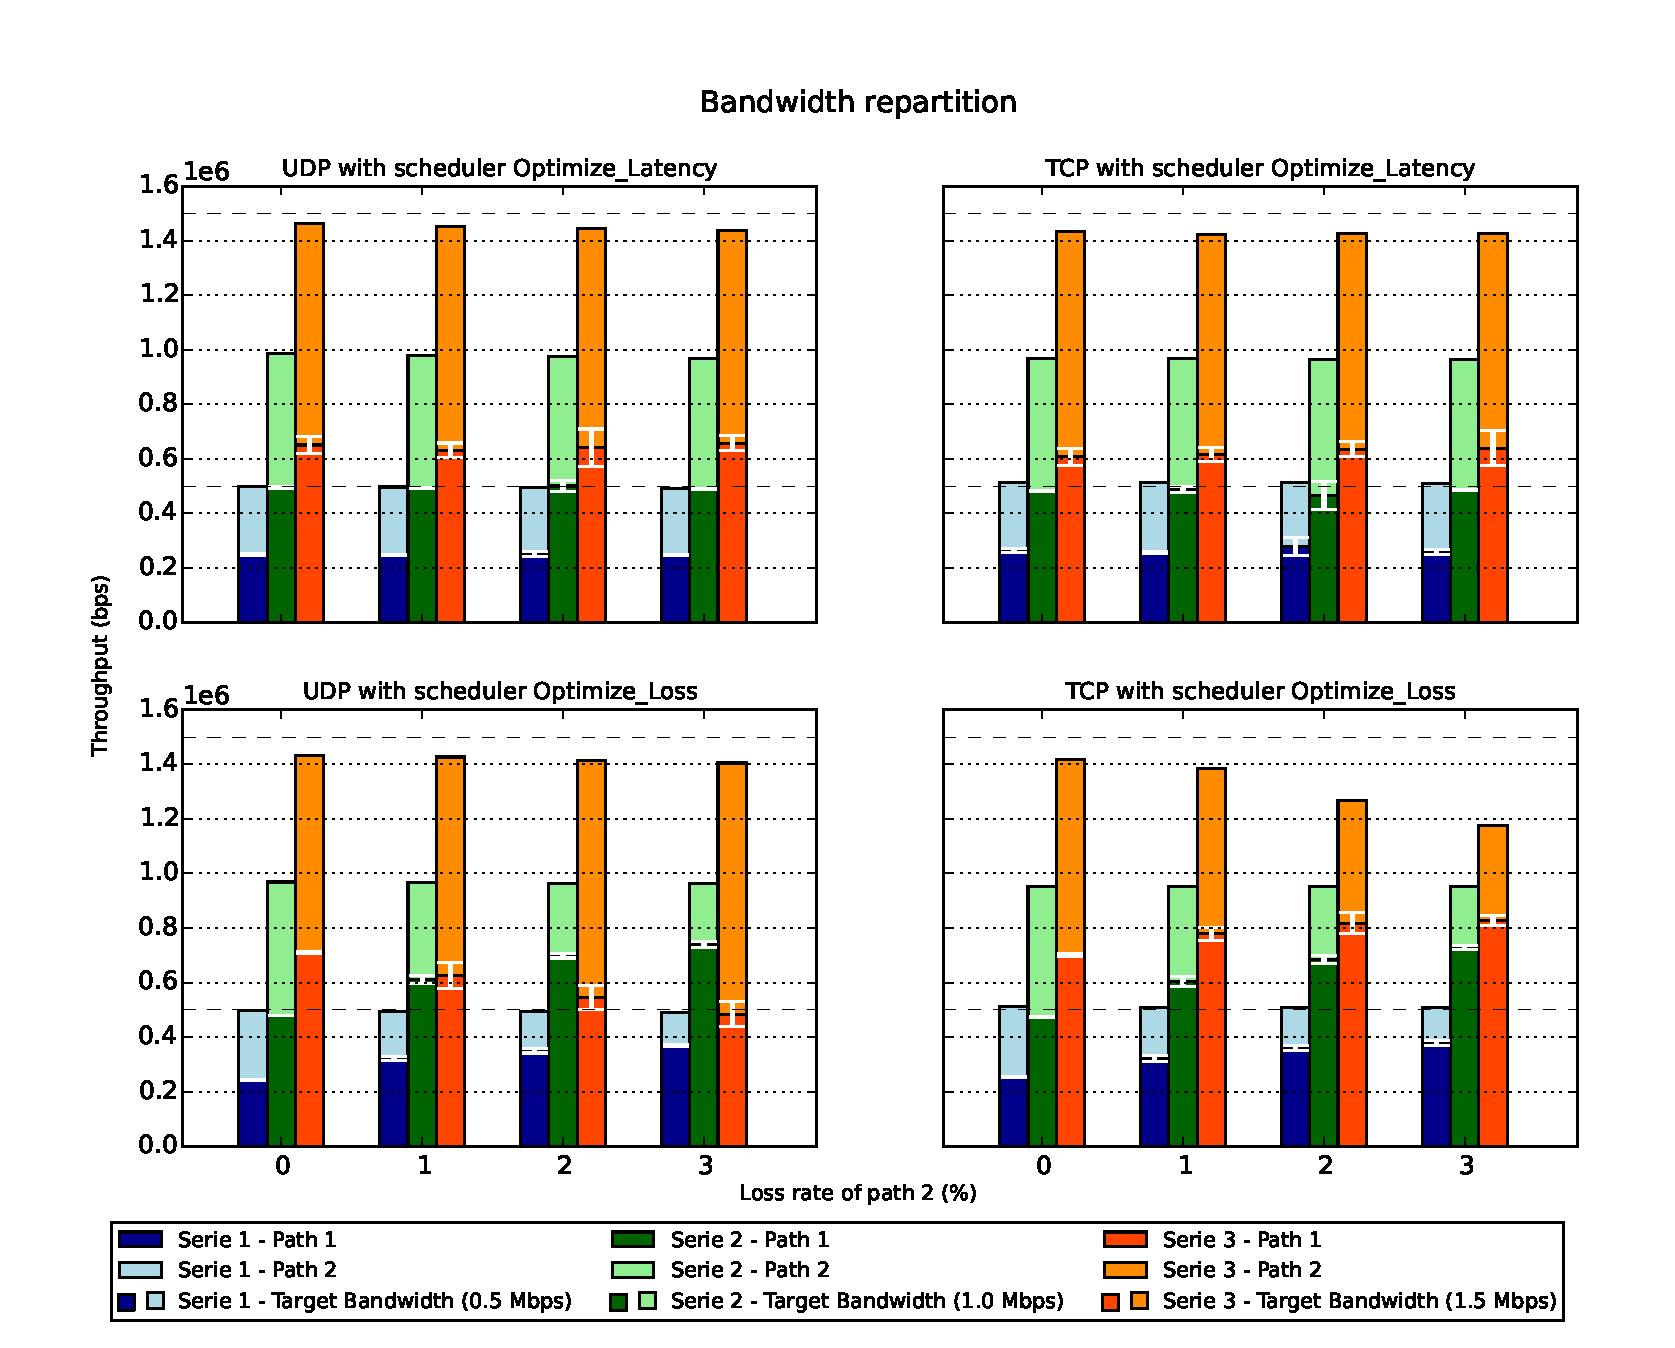
\includegraphics[width=\textwidth]{images/xp/graph2.eps}
\caption{Usage repartition with loss rate variation}
\label{fig:dynloss}
\end{figure}

A first element to point out is the fact the \texttt{Optimize Latency} scheduler is not really impacted by the loss rate as we could expect. The proportion is always around 50\% for both TCP and UDP as the two links have the same delay. The little exception to this rule is noticed for the third bar (traffic at 1.5Mbps) probably because we reach the congestion limit on path 1. Therefore, the heartbeat messages are either delayed or dropped and the forward delay is overestimated.

On the other side, the \texttt{Optimize loss} scheduler will progressively give more weight to the first path as it is loss free. We state that UDP and TCP give different results concerning the last bar which corresponds to the 1.5 Mbps transfer speed. Again, this can be explained by the congestion on path 1. UDP keeps sending packets even if they are dropped, therefore the scheduler will detect important losses on path 1. The loss rate caused by congestion will overcome the one of path 2 and the scheduler will thus choose the best option among the two. However, for TCP, the congestion control mechanism will reduce the sending rate to avoid congestion of path 1. In such conditions, path 1 remains the best option and thus receives more weight from the scheduler.


\subsection{Resiliency to interface removal}

The objective of using multipath is not only to balance the traffic on the existing paths but also to modify dynamically the distribution of the traffic if one interface becomes unavailable. For this experiment, we use the topology of Figure \ref{fig:topo-log} with the following configuration : 

\begin{table}[!ht]
\centering
\begin{tabular}{|c|c|c|c|}
\hline
Path n\degree & bandwidth & loss rate & delay  \\ \hline
1 & 5 Mbps & 0 & 10ms \\ \hline
2 & 5 Mbps & 0 & 20ms \\ \hline
3 & 5 Mbps & 0 & 40ms \\ \hline
\end{tabular}
\end{table}

We generate constant UDP traffic at 3 Mbps and observe the behavior of the implementation if path 1 is suddenly broken at $t=19s$. The bandwidth repartition is shown on Figure \ref{fig:xp-lossint-bw} and the scheduler used is \texttt{optimize loss}.


\begin{figure}[!ht]
\centering
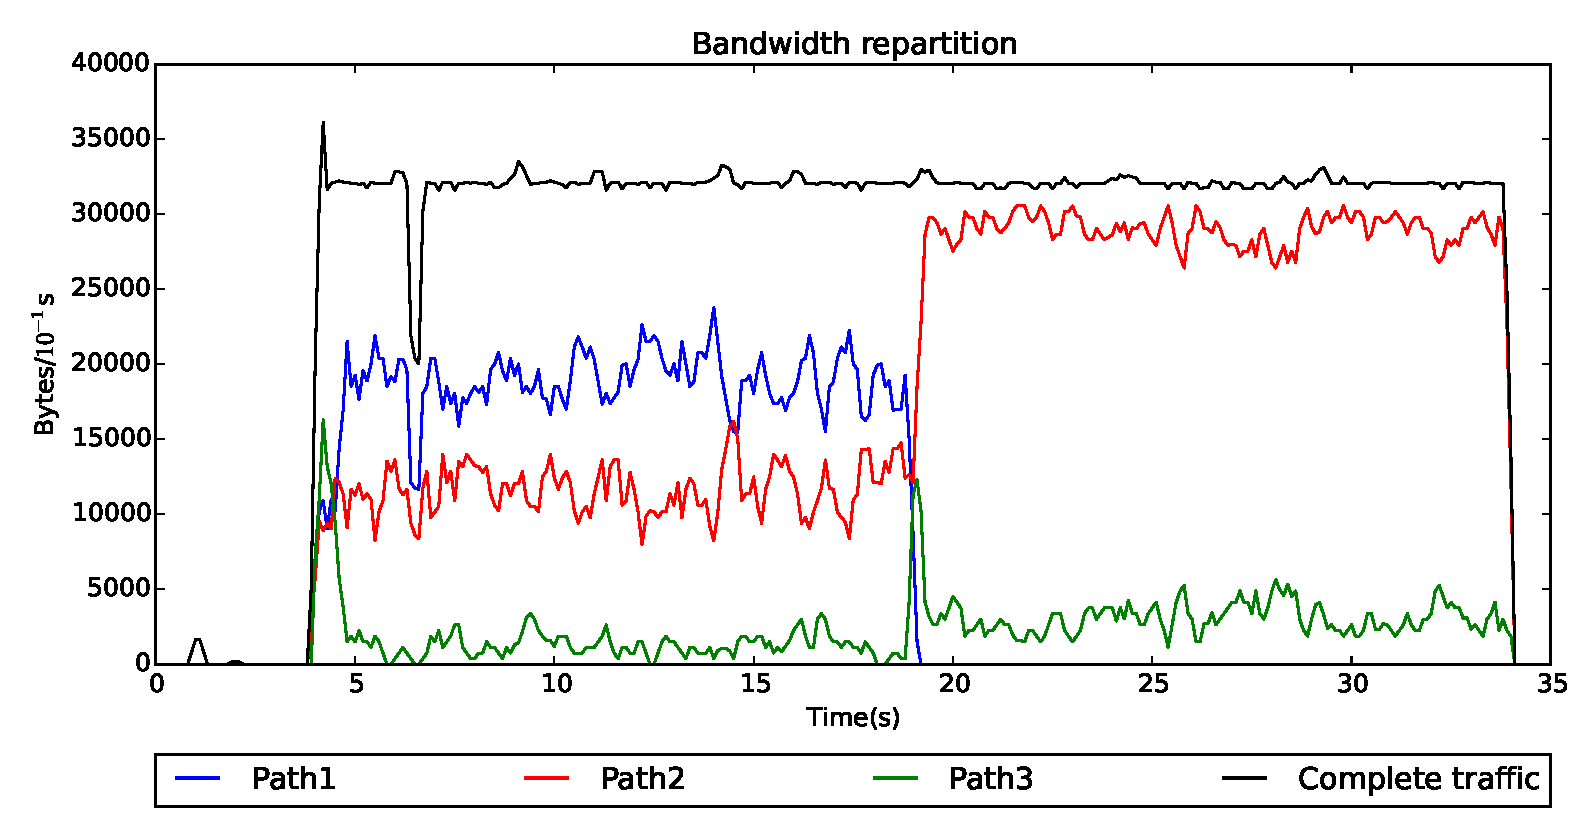
\includegraphics[width=\textwidth]{images/xp/intlost_bw.eps}
\caption{Reaction to interface removal}
\label{fig:xp-lossint-bw}
\end{figure}

Note that the path 1 was used for the handshake and we prove here that even if we remove our "primary" interface, the connection continues. In the very first moments (at 4s), we note that the distribution is more or less equal among the subflows. This setup time is needed to obtain some information about the forward delay. Heartbeat messages and feedback packets have to be exchanged between the two hosts. After 5 seconds, we see that the distribution is shaped with what we can expect from Equation \ref{eq:latency}: path 1 has almost $2/3$ of the traffic because it has the best delay, path 2 is still used because the difference of delays with path 1 is acceptable and then some traffic is given to path 3 to monitor the link. Of course, a more aggressive scheduler will probably let path 1 support 100\% of the traffic but the objective here was to use all paths to perform probing.

When path 1 fails, the distribution is recomputed and most of the traffic is re-routed to path 2. Of course we are far from the congestion because each link has a bandwidth of 5 Mbps but the objective here was to see how the distribution is moving without other constraints. In this context, the scheduler is doing well by optimizing the overall latency as we can see in Figure \ref{fig:xp-lossint-delay}. After the loss of the fastest path, the overall delay is increased and is little above the  20ms threshold which is the delay of the new fastest link. We also can observe two peaks: the first one is due to the setup time and the second one is a temporary increase of path 3 usage to compensate the failure of path 1.



\begin{figure}[!ht]
\centering
\begin{minipage}{0.4\linewidth}
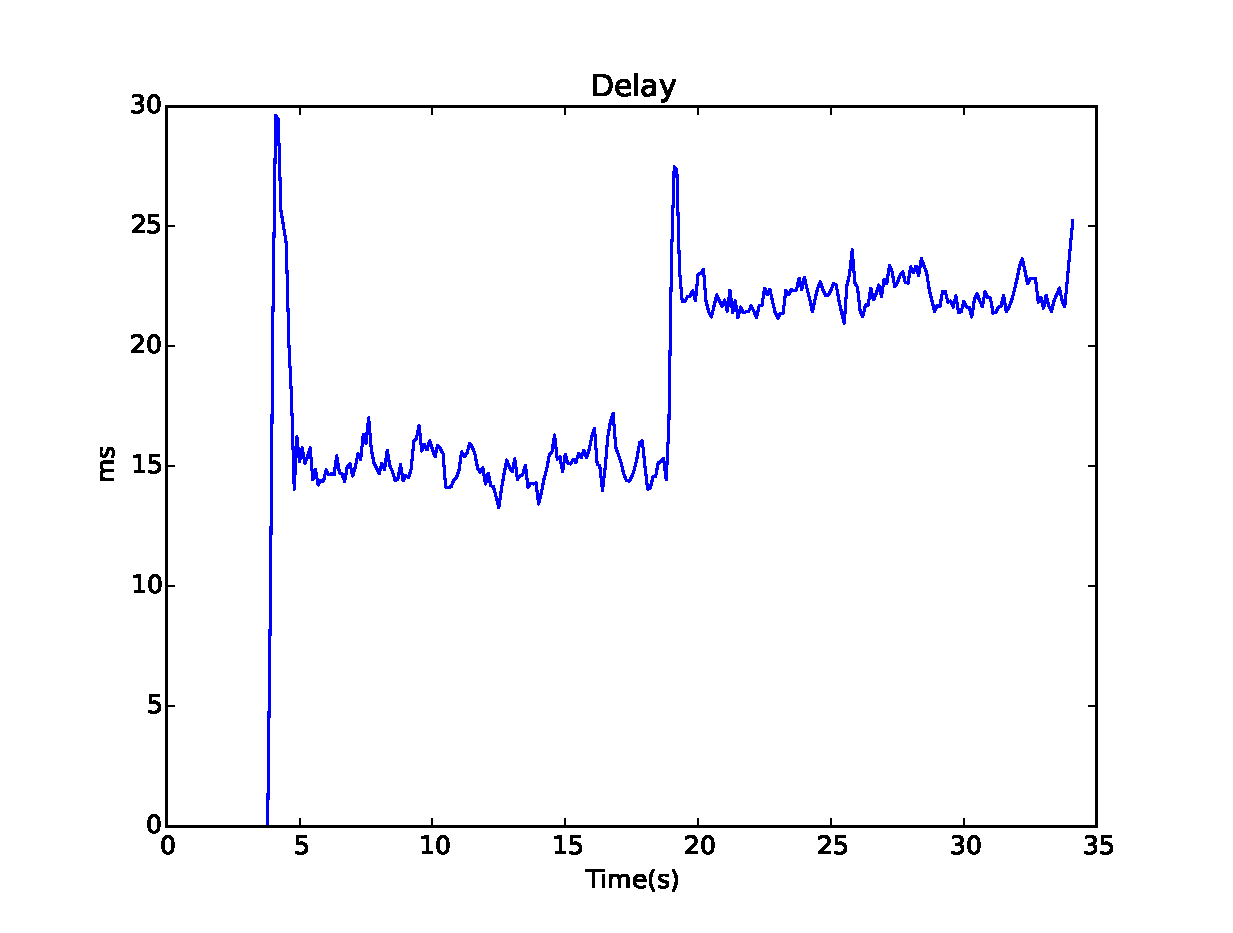
\includegraphics[width=\textwidth]{images/xp/intlost_delay.eps}
\caption{Overall delay}
\label{fig:xp-lossint-delay}
\end{minipage}
\begin{minipage}{0.59\linewidth}
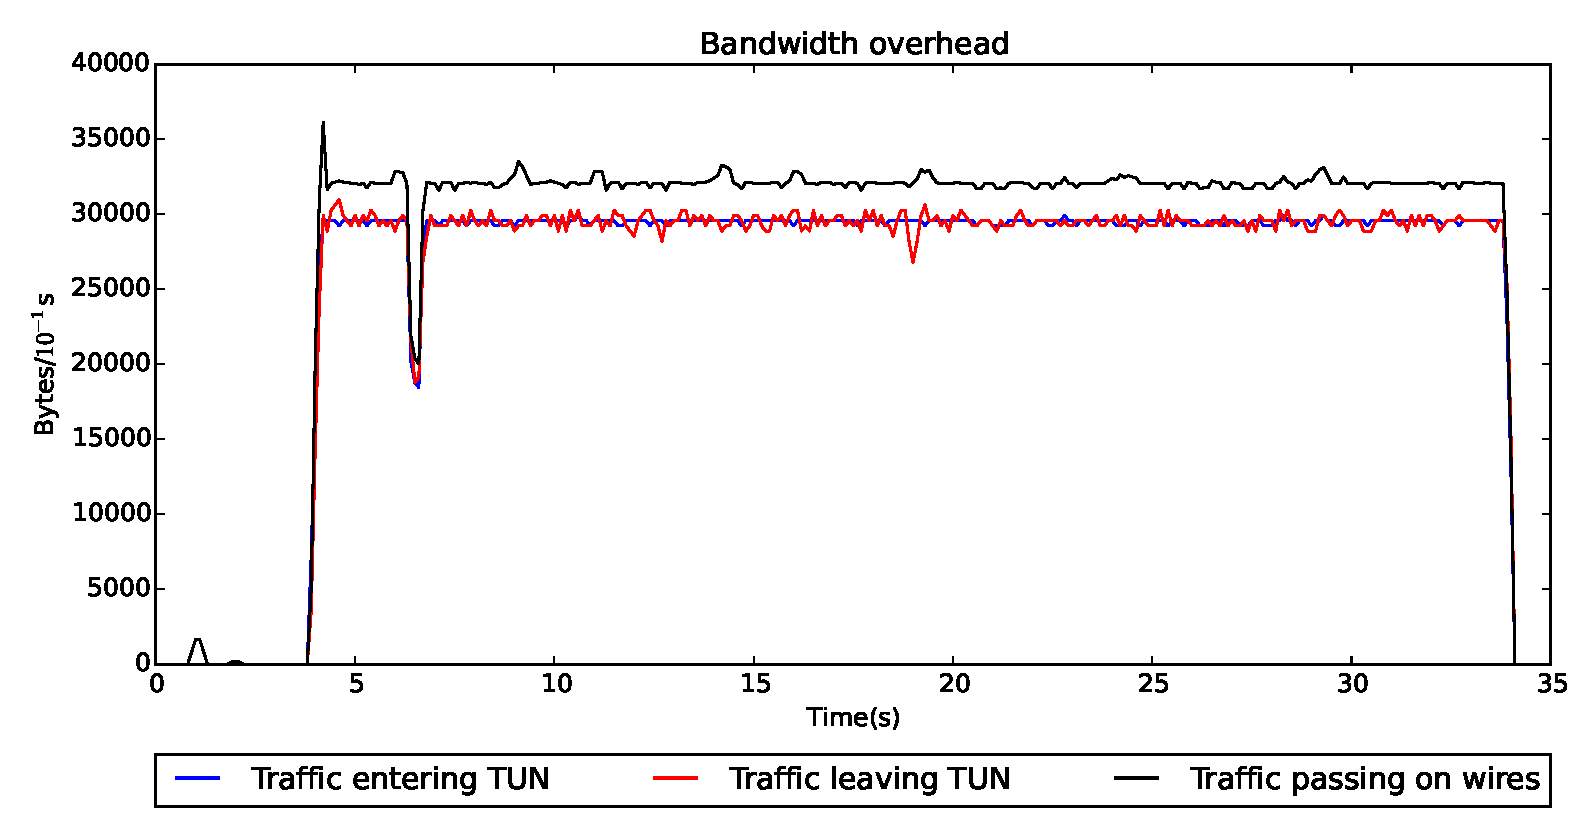
\includegraphics[width=\textwidth]{images/xp/intlost_tun.eps}
\caption{Application perception of traffic}
\label{fig:xp-lossint-tun}
\end{minipage}
\end{figure}

From the application's point of view, the impact of such failures is shown in Figure \ref{fig:xp-lossint-tun}. We see in blue the traffic entering the tunnel which is constant here because we have parametrized D-ITG to do so, in red we see the traffic leaving the tunnel and in black we have the traffic generated by the tunnel. The difference between the blue and the black curves is the overhead caused by the encapsulation of D-ITG packets inside DTLS ones. Around the $19^{th}$ second, we notice a really small drop on the red curve, exactly when the interface was lost. This is the only thing the application will perceive from the loss of one interface. This is a huge improvement in comparison with a normal DTLS connection, which would have ended the communication in case of such interface loss.

\begin{figure}[!ht]
\centering
\end{figure}

\subsection{Smooth addition of a new interface}

In this section, we explore the reverse scenario: when one interface becomes available. At the beginning only path 1 and path 2 are available and at time $t=30s$ we add path 3. The configuration used is the following :

\begin{table}[!ht]
\centering
\begin{tabular}{|c|c|c|c|}
\hline
Path n\degree & bandwidth & loss rate & delay  \\ \hline
1 & 5 Mbps & 0 & 30ms \\ \hline
2 & 5 Mbps & 0 & 40ms \\ \hline
3 & 5 Mbps & 0 & 10ms \\ \hline
\end{tabular}
\end{table}

As we can see path 3 has the lowest delay and we expect that it will take the lead over the two other ones. This is verified with our experiment as we can see on Figure \ref{fig:xp-addint-bw}. A significant portion of the traffic is redirected through the new flow. At the beginning path 1 was the fastest link so it was given the largest part. But after the addition of the new interface, a re-computation is made according to equation \ref{eq:latency} and path 1 is less used.


\begin{figure}[!ht]
\centering
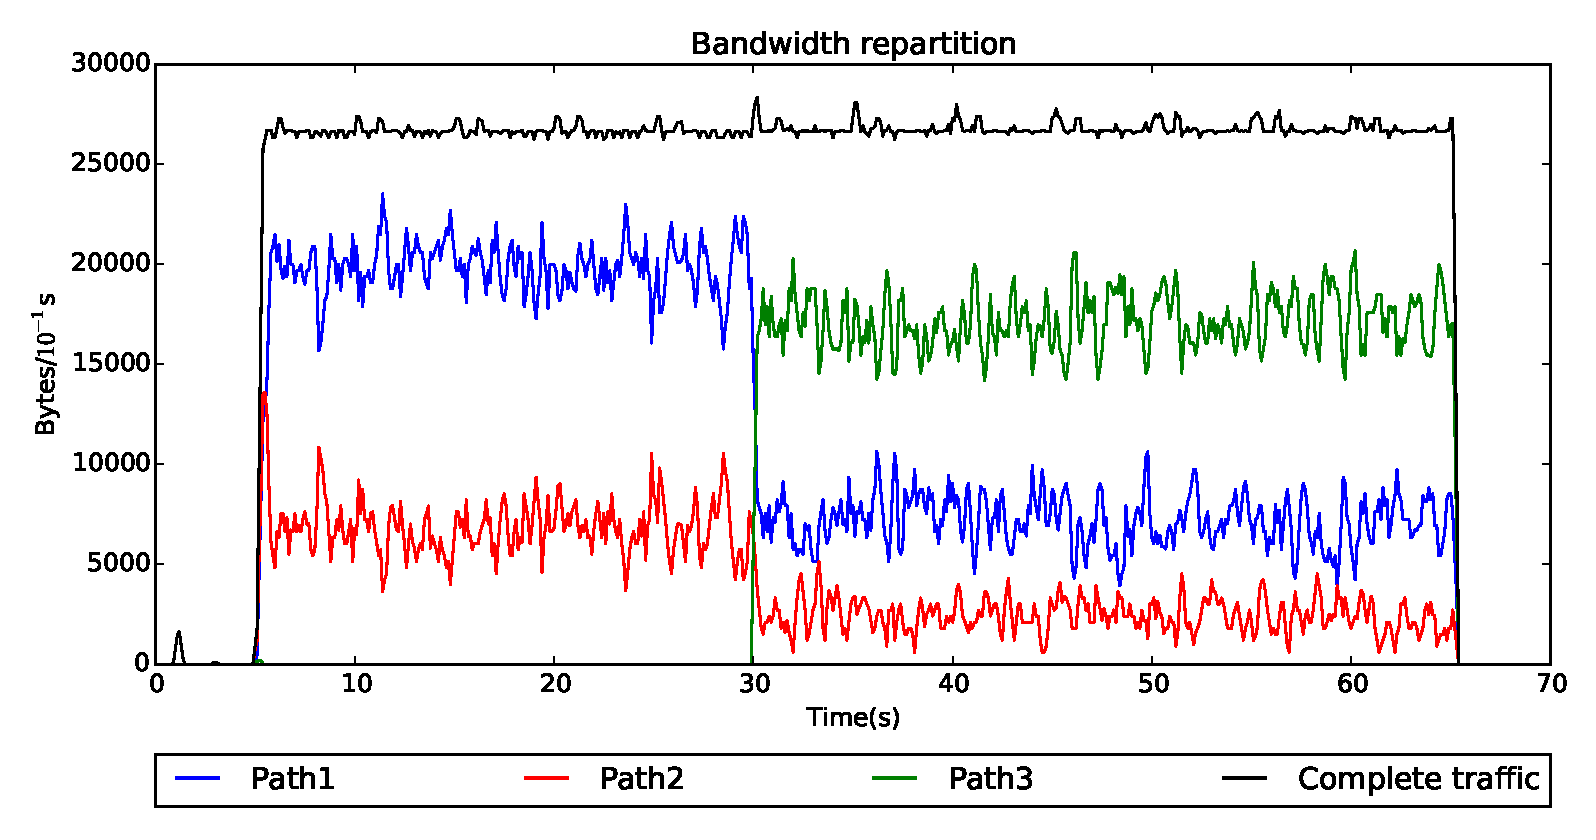
\includegraphics[width=\textwidth]{images/xp/addint_bw.eps}
\caption{Reaction to new interface addition}
\label{fig:xp-addint-bw}
\end{figure}

The overall delay is kept reasonably small according to Figure \ref{fig:xp-addint-delay} but we could probably optimize even more. That would imply putting more weight to path 1 and thus offloading the two other flows. However this is a choice we made to keep using all the paths while still trying to give more traffic to the faster link. It allows faster recovery if the best interface is lost.

\begin{figure}[!ht]
\centering
\begin{minipage}{0.4\linewidth}
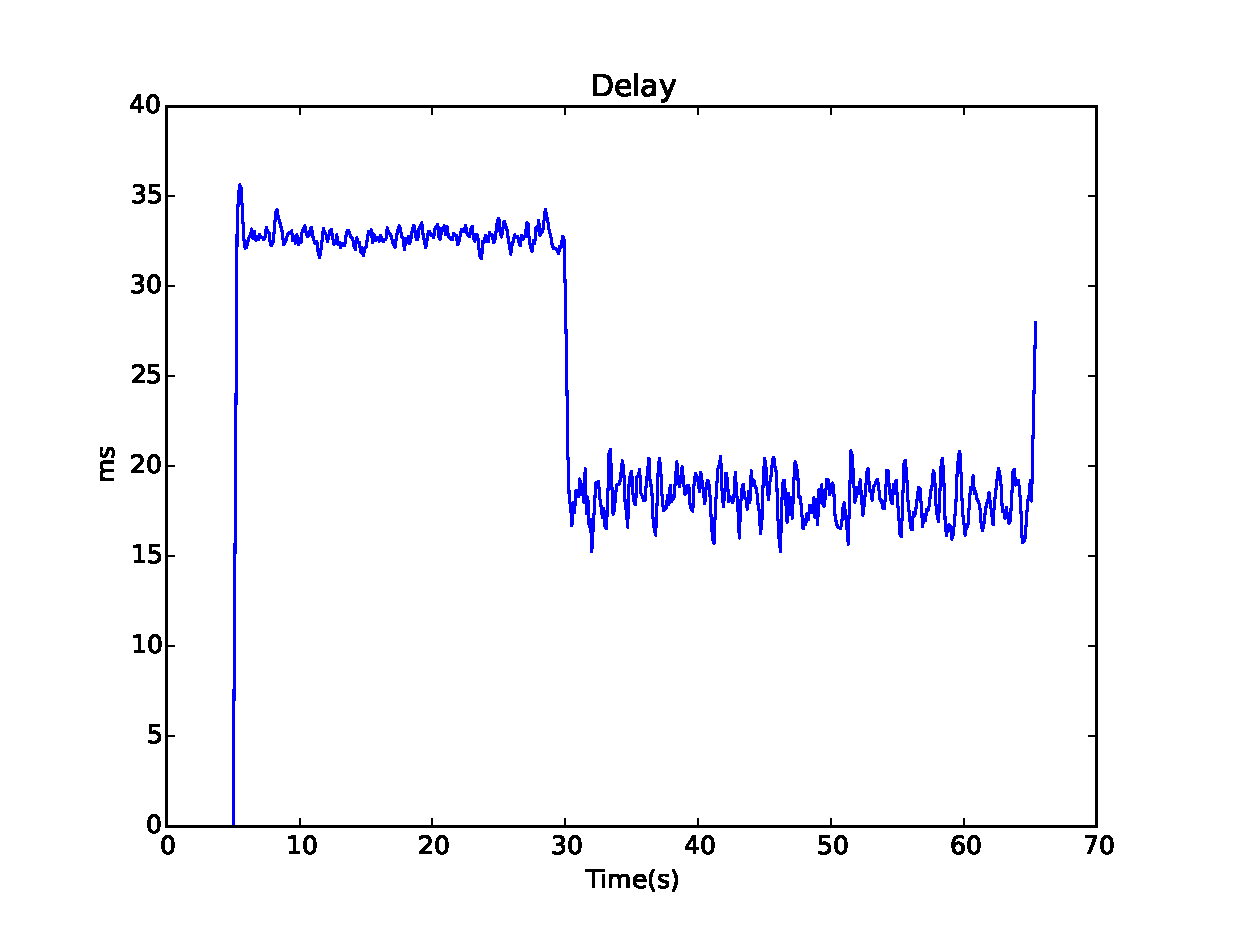
\includegraphics[width=\textwidth]{images/xp/addint_delay.eps}
\caption{Overall delay}
\label{fig:xp-addint-delay}
\end{minipage}
\begin{minipage}{0.59\linewidth}
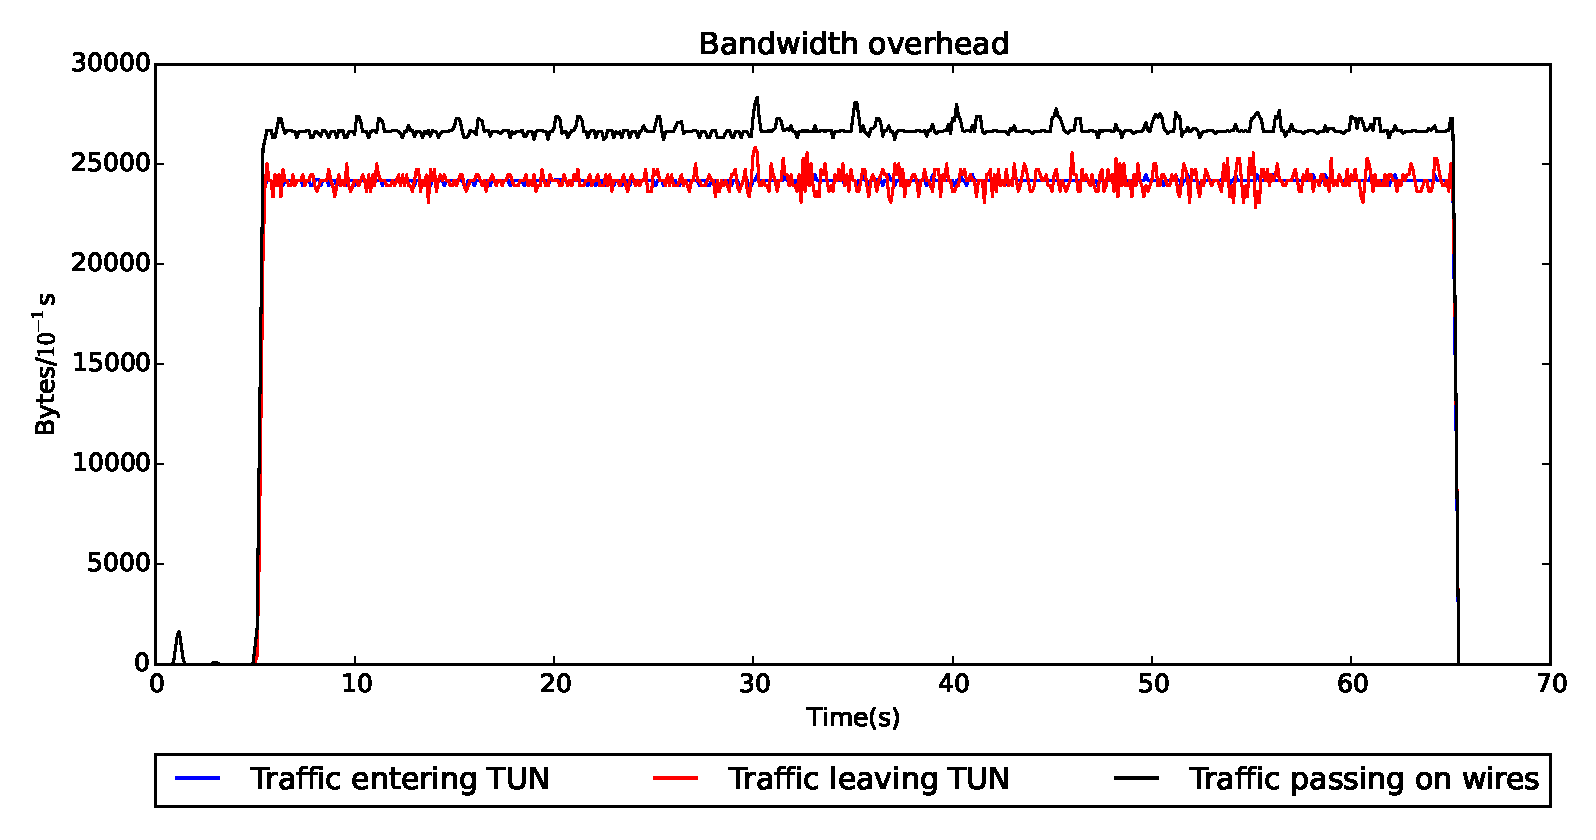
\includegraphics[width=\textwidth]{images/xp/addint_tun.eps}
\caption{Application perception of traffic}
\label{fig:xp-addint-tun}
\end{minipage}
\end{figure}

If we look at the traffic perceived by the application on Figure \ref{fig:xp-addint-tun}, we notice no real perturbation around $30s$. Although the traffic is a bit noisy after this time, this is explained by the fact we have 3 different paths with 3 different delays and therefore packets cannot arrive at a constant rate.

\section{Conclusion}

In this chapter, we have presented a simple VPN application that we have designed to evaluate our MPDTLS implementation. To dispatch efficiently the packets between the available flows, 3 schedulers have been created : \texttt{Round Robin}, \texttt{Optimize Loss} and \texttt{Optimize Latency}. We have concentrated our evaluation on the last two since the \texttt{Round Robin} doesn't consider any contextual information. 

After various experiments, we have shown that the \texttt{Optimize Latency} scheduler behaves better when there is no congestion. Otherwise, it tries to push a large amount of traffic on the faster link and quickly triggers congestion. However, we have discovered that the counter-reaction will avoid too many losses. As the additional delay caused by the congestion will increase the perceived latency, the scheduler will therefore redirect the traffic through other paths.

On the other side, the \texttt{Optimize Loss} scheduler behaves better when there is congestion or simply if one link looses more packets than another one. This would typically be the case for a Wi-Fi interface in an environment with interference. In such case, the most reliable link is preferred as long as it is not congested.

In addition, we have shown that an application using our MPDTLS tunnel will not be much troubled if one interface is lost in the middle of the communication. This is also the case if we add a new interface on the fly.






 
\if0\draft

\chapter*{Conclusion\markboth{Conclusion}{}}
\addcontentsline{toc}{chapter}{Conclusion}
\appendix

\fi
\bibliographystyle{unsrt}
\bibliography{articles,rfcs}

\end{document}

